% Options for packages loaded elsewhere
\PassOptionsToPackage{unicode}{hyperref}
\PassOptionsToPackage{hyphens}{url}
%
\documentclass[
  12pt,
  letterpaper,
]{article}
\usepackage{amsmath,amssymb}
\usepackage{setspace}
\usepackage{iftex}
\ifPDFTeX
  \usepackage[T1]{fontenc}
  \usepackage[utf8]{inputenc}
  \usepackage{textcomp} % provide euro and other symbols
\else % if luatex or xetex
  \usepackage{unicode-math} % this also loads fontspec
  \defaultfontfeatures{Scale=MatchLowercase}
  \defaultfontfeatures[\rmfamily]{Ligatures=TeX,Scale=1}
\fi
\usepackage{lmodern}
\ifPDFTeX\else
  % xetex/luatex font selection
\fi
% Use upquote if available, for straight quotes in verbatim environments
\IfFileExists{upquote.sty}{\usepackage{upquote}}{}
\IfFileExists{microtype.sty}{% use microtype if available
  \usepackage[]{microtype}
  \UseMicrotypeSet[protrusion]{basicmath} % disable protrusion for tt fonts
}{}
\makeatletter
\@ifundefined{KOMAClassName}{% if non-KOMA class
  \IfFileExists{parskip.sty}{%
    \usepackage{parskip}
  }{% else
    \setlength{\parindent}{0pt}
    \setlength{\parskip}{6pt plus 2pt minus 1pt}}
}{% if KOMA class
  \KOMAoptions{parskip=half}}
\makeatother
\usepackage{xcolor}
\usepackage[top=2.5cm, bottom=2.5cm, left=3.5cm, right=3.5cm]{geometry}
\usepackage{longtable,booktabs,array}
\usepackage{calc} % for calculating minipage widths
% Correct order of tables after \paragraph or \subparagraph
\usepackage{etoolbox}
\makeatletter
\patchcmd\longtable{\par}{\if@noskipsec\mbox{}\fi\par}{}{}
\makeatother
% Allow footnotes in longtable head/foot
\IfFileExists{footnotehyper.sty}{\usepackage{footnotehyper}}{\usepackage{footnote}}
\makesavenoteenv{longtable}
\usepackage{graphicx}
\makeatletter
\def\maxwidth{\ifdim\Gin@nat@width>\linewidth\linewidth\else\Gin@nat@width\fi}
\def\maxheight{\ifdim\Gin@nat@height>\textheight\textheight\else\Gin@nat@height\fi}
\makeatother
% Scale images if necessary, so that they will not overflow the page
% margins by default, and it is still possible to overwrite the defaults
% using explicit options in \includegraphics[width, height, ...]{}
\setkeys{Gin}{width=\maxwidth,height=\maxheight,keepaspectratio}
% Set default figure placement to htbp
\makeatletter
\def\fps@figure{htbp}
\makeatother
\setlength{\emergencystretch}{3em} % prevent overfull lines
\providecommand{\tightlist}{%
  \setlength{\itemsep}{0pt}\setlength{\parskip}{0pt}}
\setcounter{secnumdepth}{-\maxdimen} % remove section numbering
% definitions for citeproc citations
\NewDocumentCommand\citeproctext{}{}
\NewDocumentCommand\citeproc{mm}{%
  \begingroup\def\citeproctext{#2}\cite{#1}\endgroup}
\makeatletter
 % allow citations to break across lines
 \let\@cite@ofmt\@firstofone
 % avoid brackets around text for \cite:
 \def\@biblabel#1{}
 \def\@cite#1#2{{#1\if@tempswa , #2\fi}}
\makeatother
\newlength{\cslhangindent}
\setlength{\cslhangindent}{1.5em}
\newlength{\csllabelwidth}
\setlength{\csllabelwidth}{3em}
\newenvironment{CSLReferences}[2] % #1 hanging-indent, #2 entry-spacing
 {\begin{list}{}{%
  \setlength{\itemindent}{0pt}
  \setlength{\leftmargin}{0pt}
  \setlength{\parsep}{0pt}
  % turn on hanging indent if param 1 is 1
  \ifodd #1
   \setlength{\leftmargin}{\cslhangindent}
   \setlength{\itemindent}{-1\cslhangindent}
  \fi
  % set entry spacing
  \setlength{\itemsep}{#2\baselineskip}}}
 {\end{list}}
\usepackage{calc}
\newcommand{\CSLBlock}[1]{\hfill\break\parbox[t]{\linewidth}{\strut\ignorespaces#1\strut}}
\newcommand{\CSLLeftMargin}[1]{\parbox[t]{\csllabelwidth}{\strut#1\strut}}
\newcommand{\CSLRightInline}[1]{\parbox[t]{\linewidth - \csllabelwidth}{\strut#1\strut}}
\newcommand{\CSLIndent}[1]{\hspace{\cslhangindent}#1}
\ifLuaTeX
\usepackage[bidi=basic]{babel}
\else
\usepackage[bidi=default]{babel}
\fi
\babelprovide[main,import]{spanish}
% get rid of language-specific shorthands (see #6817):
\let\LanguageShortHands\languageshorthands
\def\languageshorthands#1{}
\usepackage{fontspec}
\setmainfont{Arial}
\usepackage{tocloft}
\usepackage{floatrow}
\usepackage{caption}
\AtBeginDocument{\renewcommand{\listtablename}{Índice de Tablas}}
\AtBeginDocument{\renewcommand{\listfigurename}{Índice de Figuras}}
\AtBeginDocument{\renewcommand{\tablename}{Tabla}}
\AtBeginDocument{\renewcommand{\figurename}{Figura}}
\renewcommand{\cftfigpresnum}{Figura~}
\renewcommand{\cftfigaftersnum}{:\quad}
\renewcommand{\cfttabpresnum}{Tabla~}
\renewcommand{\cfttabaftersnum}{:\quad}
\cftsetindents{figure}{1.5em}{4.75em}
\cftsetindents{table}{1.5em}{4em}
\DeclareCaptionLabelFormat{apa}{\textbf{#1~#2}\\}
\captionsetup[figure]{labelformat=apa, textfont=it, name=Figura, labelsep=none, justification=raggedright, singlelinecheck=false}
\captionsetup[table]{labelformat=apa, textfont=it, name=Tabla, labelsep=none, justification=raggedright, singlelinecheck=false}
\floatsetup[figure]{capposition=top}
\floatsetup[table]{capposition=top}
\floatplacement{figure}{H}
\floatplacement{table}{H}
\usepackage{booktabs}
\usepackage{longtable}
\usepackage{array}
\usepackage{multirow}
\usepackage{wrapfig}
\usepackage{float}
\usepackage{colortbl}
\usepackage{pdflscape}
\usepackage{tabu}
\usepackage{threeparttable}
\usepackage{threeparttablex}
\usepackage[normalem]{ulem}
\usepackage{makecell}
\usepackage{xcolor}
\ifLuaTeX
  \usepackage{selnolig}  % disable illegal ligatures
\fi
\usepackage{bookmark}
\IfFileExists{xurl.sty}{\usepackage{xurl}}{} % add URL line breaks if available
\urlstyle{same}
\hypersetup{
  pdflang={es},
  hidelinks,
  pdfcreator={LaTeX via pandoc}}

\author{}
\date{\vspace{-2.5em}}

\begin{document}

\setstretch{1}
\begin{titlepage}
    \begin{flushleft}
        \vspace{2.5cm}
        \begin{minipage}{0.7\textwidth}
            {\fontsize{14}{14}\selectfont \textbf{UNIVERSIDAD DE SANTIAGO DE CHILE}} \\[0.2cm]
            {\fontsize{12}{12}\selectfont \textbf{FACULTAD DE ADMINISTRACIÓN Y ECONOMÍA}} \\[0.2cm]
            {\fontsize{12}{12}\selectfont \textbf{Departamento de Gestión y Políticas Públicas}}
        \end{minipage}
        \hfill
        \begin{minipage}{0.2\textwidth}
            \centering
            
\includegraphics[width=3.5cm]{archivos/logo_usach.png}
        \end{minipage}
    \end{flushleft}

    \vspace{3cm}

    \begin{center}
        {\fontsize{12}{12}\selectfont \textbf{Desmunicipalización y gestión educativa: un estudio sobre la implementación de los Servicios Locales de Educación Pública}} \\[5.5cm]

        {\fontsize{12}{12}\selectfont \textbf{Autor:} Nicolás Torres Hormazábal} \\[2cm]
    \end{center}

    \begin{flushright}
        {\fontsize{12}{12}\selectfont \textbf{Profesor Guía:} Ignacio Larraguibel} \\[1cm]

        {\fontsize{12}{12}\selectfont 
        \textbf{Tesis para optar al grado académico de} \\
        \textbf{Licenciado en Administración Pública}} \\[2cm]
    \end{flushright}

    \begin{center}
        {\fontsize{12}{12}\selectfont Santiago – Chile} \\[0.3cm]
        {\fontsize{12}{12}\selectfont 2025}  
    \end{center}
\end{titlepage}
\newpage
\begin{titlepage}
  \vspace*{\fill}

  \begin{flushleft}
    {\fontsize{12}{14}\selectfont
    \textbf{
      © Nicolás Felipe Torres Hormazábal, 2025 \\[0.3cm]
      Esta obra está bajo una Licencia Creative Commons \\[0.3cm]
      Reconocimiento Internacional 4.0
    } \\[0.5cm]
    
\includegraphics[width=3cm]{archivos/logo_cc.png}
    }
  \end{flushleft}

  \vspace*{0.5cm}
\end{titlepage}

\newpage
\clearpage
\newpage

\noindent\textbf{\Large Dedicatoria}

Para mis padres y familia, quienes siempre me han apoyado en todas mis decisiones -sin cuestionar- y me han apoyado y dado tranquilidad para poder estudiar.

A mi amada Rocío, a quien admiro cada día más.

A mis dos perros y dos gatos, a quienes amo demasiado y me entregan paz sin saberlo.

A mi abuela, Ana (Q.E.P.D), a quien considero una segunda madre y extraño cada día.

Y a todos mis seres amados.
Ustedes saben quiénes son.

\clearpage
\newpage

\noindent\textbf{\Large Agradecimientos}

Quiero agradecer a todas aquellas personas que en mayor o menor medida contribuyeron a que esté finalizando mi proceso universitario.
A todos aquellos con quienes hablé de manera casual, con quienes hice trabajo en grupo o con quienes tuve una amistad más profunda.
Por escuchar mis problemas o simplemente distender.

De igual manera, agradezco la oportunidad de haber cursado el \emph{minor} en Ciencia de Datos de la Facultad de Ingeniería, que me entregó una mirada distinta del mundo y donde pude aprender muchos conceptos y técnicas de \emph{software} que fueron aplicados en este trabajo.
A todos los profesores y quienes trabajan en ese programa, muchas gracias por la paciencia y la disposición a enseñar.

También a mi profesor guía, Ignacio Larraguibel, cuyos comentarios y ayuda en general fueron un gran aporte para finalizar de manera conforme este documento.

Finalmente, a Nicanor Parra y su famosa observación, frase o pensamiento -que no sé si es de él, pero que siempre se le atribuye- que versa:

\begin{quote}
\emph{Hay dos panes. Usted se come dos. Yo ninguno. Consumo promedio: un pan por persona}
\end{quote}

la que me hizo cuestionar muchas cifras y estadísticas y despertó mi curiosidad por entender cómo funcionaban.

\clearpage
\newpage
\tableofcontents
\clearpage
\newpage
\listoftables
\clearpage
\newpage
\listoffigures
\clearpage
\newpage

\section{Resumen}\label{resumen}

Este estudio presenta un análisis cuantitativo con enfoque exploratorio sobre los Servicios Locales de Educación Pública (SLEP) en Chile, con el objetivo de identificar patrones en su estructura y desempeño.
Se busca comprender cómo operan los establecimientos traspasados desde la administración municipal, evaluando variables académicas, docentes y socioeconómicas.

La metodología se basa en técnicas de ciencia de datos, utilizando Análisis de Componentes Principales (PCA) para reducir la dimensionalidad y el algoritmo K-Means para clasificar establecimientos según similitudes.
Las variables consideradas incluyen matrícula, resultados del Sistema de Medición de la Calidad de la Educación (SIMCE), carga laboral docente, dotación de asistentes de la educación y nivel de vulnerabilidad socioeconómica.

Los resultados permiten agrupar los establecimientos en tres categorías distintas, mostrando relaciones entre rendimiento académico, exigencia docente y distribución de recursos.
También se evidencian diferencias territoriales y socioeconómicas que afectan la calidad del servicio educativo.

Esta investigación contribuye al monitoreo temprano de la implementación de la Ley N.º 21.040, entregando evidencia empírica útil para la toma de decisiones en política educativa.
Sus hallazgos permiten visibilizar la diversidad interna del sistema público y orientar estrategias que fortalezcan la gestión, la equidad y la calidad de la educación en el marco de la Nueva Educación Pública.

\textbf{Palabras clave:} \emph{Servicios Locales de Educación Pública (SLEP), análisis cuantitativo, K-Means, PCA, vulnerabilidad socioeconómica, equidad educativa}

\newpage

\section{Introducción}\label{introducciuxf3n}

A lo largo de la historia de Chile, la educación pública ha pasado por varios momentos claves, desde la fundación de las escuelas normales a mediados del siglo XIX, la fundación del Ministerio de Educación (MINEDUC) en 1927, que profundizó los lazos del Estado chileno con la educación pública, consolidándose el llamado Estado docente, hasta los radicales cambios que experimentó durante la dictadura militar y su profundización durante el retorno a la democracia.

Este modelo, basado en la descentralización y una lógica de mercado, ha sido criticado por su incapacidad para reducir las desigualdades educativas y asegurar una calidad homogénea en el sistema educativo, generando profundas brechas entre comunas y regiones de diferentes niveles socioeconómicos (Baleriola et~al., 2021).

En respuesta a estas limitaciones, la Ley N.º 21.040, promulgada en 2017, marca un cambio de paradigma en la gestión de la educación pública chilena al establecer los nuevos paradigmas de la educación pública al crear los Servicios Locales de Educación Pública (Biblioteca del Congreso Nacional de Chile, 2017).

Los SLEP representan un nivel intermedio de administración que transfiere la gestión de los establecimientos desde los municipios hacia este nuevo nivel intermedio.
Este modelo tiene como objetivo profesionalizar la administración, optimizar el uso de los recursos y garantizar que todos los estudiantes, independientemente de su ubicación geográfica o condición socioeconómica, tengan acceso a una educación de calidad (Bellei, 2018).

La siguiente investigación busca conocer y comprender los impactos que ha tenido la implementación la ley 21.040 en distintos SLEP seleccionados, desde concretado su traspaso de municipal a Servicio Local.
Para esto, se usarán métodos cuantitativos como agrupamiento de datos, con el fin de encontrar características, patrones u otros descubrimientos que puedan compartir los establecimientos de distintas comunas, nutriéndose de las bases de datos del MINEDUC y otras fuentes gubernamentales, específicamente las referidas a docentes y asistentes de la educación, ruralidad, características socioeconómicas de los alumnos y establecimientos, y finalmente, resultados de pruebas estandarizadas.

\newpage

\section{Antecedentes}\label{antecedentes}

La educación pública constituye uno de los pilares esenciales del Estado, no solo por su función en la transmisión de conocimientos académicos, sino también por su capacidad para promover la equidad social, la cohesión comunitaria y el desarrollo integral de las personas.
Como servicio provisto por el Estado, ha sido históricamente una herramienta para ampliar oportunidades, reducir desigualdades y formar ciudadanos capaces de desenvolverse en sociedad.

\subsection{La educación pública en Chile}\label{la-educaciuxf3n-puxfablica-en-chile}

En Chile, el sistema de educación pública ha cumplido un rol clave en la construcción del Estado moderno.
Desde sus orígenes, ha buscado garantizar el acceso al conocimiento como un derecho social, permitiendo que niñas, niños y adolescentes accedan a una formación común sin importar su origen territorial o condición socioeconómica.

Esta misión se ha traducido en esfuerzos sostenidos por ampliar la cobertura escolar, erradicar el analfabetismo y consolidar una estructura pública que asegure el ejercicio continuo y universal de este derecho.

Lo anterior da cuenta del compromiso que ha tenido el Estado de Chile con la educación a lo largo de su historia, que tiene sus bases actuales en la creación del Ministerio de Educación en 1927.
Es en este período donde nace el llamado ``Estado Docente'', concepto acuñado para dar nombre a ese conjunto de normas y nociones sobre el rol principal que el Estado debe tener al proveer educación para la población.

Con este primer gran hito, se consolida la educación pública como ``centralizada, altamente burocrática y jerárquica'' (Bellei, 2018, p. 22), conceptos propios de organizaciones de inicios del siglo pasado, pero que a pesar de todo dieron frutos.
El objetivo de estas medidas era poner a disposición de los ciudadanos la educación con el fin de aumentar el capital humano del país, persiguiendo el desarrollo académico y espiritual de las personas.
Aunque su estructura organizacional tan centralizada resultaba laboriosa de administrar, además, no se puede obviar las condiciones del país durante esos años, con menor acceso a servicios básicos como salud y trabajo decente.
A pesar de esto, los esfuerzos por lograr la escolaridad dieron frutos.

El objetivo principal de la educación primaria y secundaria ha sido siempre formar al mayor número de ciudadanos posible, bajo la premisa de que mejores condiciones educativas conducen al progreso individual y nacional.
La existencia de distintos tipos de educación y el acceso gratuito a escuelas desde una edad temprana reflejan el compromiso del Estado en facilitar este derecho.

En los inicios del sistema educacional chileno, la principal preocupación era la expansión de la cobertura escolar, sin mayor énfasis en los mecanismos administrativos.
Un claro ejemplo de esto fueron los profesores normalistas, quienes fueron los primeros profesores con conocimientos avanzados y superiores de materias y pedagogía, siendo así pilares fundamentales del sistema educativo de la época, y sentaron las bases para la enseñanza en Chile (Memoria Chilena, s.~f.)

\subsection{Transformaciones en el sistema educativo chileno}\label{transformaciones-en-el-sistema-educativo-chileno}

Uno de los cambios más significativos en la educación pública chilena ocurrió durante la dictadura, cuando se redefinió el rol del Estado en la educación y, más importante aún, se modificó la forma en que debía proveerse, financiarse y administrarse.

Es entonces donde nace la municipalización de la educación en nuestro país, que es un traspaso de facultades de administración de un nivel centralizado como lo era anteriormente, por medio del Ministerio, hacia un nuevo nivel descentralizado, donde las municipalidades y la administración local son los nuevos responsables de su funcionamiento (Garretón et~al., 2022, p. 5).
Este proceso como la mayoría de los radicales cambios que afectaron al sistema estatal chileno durante esta época se dio de manera autoritaria, con lo que no hubo una resistencia o miradas distintas a este proceso.

Las inspiraciones detrás de este nuevo sistema tienen directa relación con lógicas de mercado, y con un entendimiento de la educación como ``un bien individual y consumible'' (Locatelli, 2018, p. 184).
En este período nació el financiamiento tipo \emph{voucher} que se manifestó en forma de subvenciones a proveedores y sostenedores de la educación, aunque este pago resulta ser el mismo para colegios municipales como subvencionados, con lo que en la práctica deja en desmedro a las familias con menos recursos, y beneficia a quienes si pueden elegir su proyecto educativo (Bellei, 2018, p. 23).

Esta lógica de mercado incentivó una competitividad entre establecimientos municipales y subvencionados; el hecho de tener una subvención por asistencia crea incentivos para los colegios de captar alumnos como sea, con lo que se deja en desmedro a la educación totalmente pública, y también se debilita al nivel central que durante este período solamente era un ente que veía como la educación iba cambiando a medida que cambiaba la demanda, por otra parte, las escuelas públicas no podían competir de igual a igual con las subvencionadas ya que, entre otras razones que no abordaremos en este análisis, los recursos que manejaban eran menores, así como de poseer una legislación más rigurosa (Bellei, 2018, p. 24).

El tiempo pasó y las notorias diferencias propias de un sistema regido por lógicas de mercado se hizo cada vez más evidente, la segregación y fallas del sistema, normas heredadas de la dictadura (como la Ley Orgánica Constitucional de Educación (LOCE)) generaban malestar en la sociedad, y sobre todo en los estudiantes secundarios.
Esto se demostró en la ``revolución pingüina'', durante 2006 (Bellei et~al., 2010, pp. 12-13).

Cinco años después, durante el 2011 también hubo protestas respecto al estado de la educación, aunque estas estaban más enfocadas al lucro en la educación superior.
El sistema educativo chileno tenía evidentes problemas, que requieren solución (Bellei, 2018, p. 37).
En este turbulento proceso, es que se empezaron a abordar distintas soluciones al problema de la educación primaria y secundaria, y es aquí donde nacen las nociones que luego darían lugar a la ley 21.040 sobre la Nueva Educación Pública (NEP) y los SLEP.

\subsection{Nacimiento de la Nueva Educación Pública y los SLEP}\label{nacimiento-de-la-nueva-educaciuxf3n-puxfablica-y-los-slep}

Como se ha mencionado, la ley sobre los SLEP y NEP fue promulgada en 2017, y empezó a aplicarse desde el año siguiente.
Es una medida reciente, y el proceso denominado como ``desmunicipalización'', esto es, traspasar las facultades administrativas de las municipales o corporaciones de educación hacia el nuevo organismo de nivel intermedio llamado SLEP, todavía se está llevando a cabo (Biblioteca del Congreso Nacional de Chile, 2017).

Al 1 de enero de 2025, 9 nuevos Servicios Locales entraron en funcionamiento: Licanbur, Los Libertadores, Santa Corina, Santa Rosa, Del Pino, Maule Costa, Andalién Costa, Valdivia y Chiloé.
Estos se suman a los 15 que ya estaban en funcionamiento, teniendo un total de 24 SLEP operativos en todo el país (Ministerio de Educación, 2024).

Este proceso no ha estado exento de dificultades y críticas por su funcionamiento y puesta en marcha, tanto por integrantes de los SLEP como externos a ellos.

Un estudio realizado en los primeros años de funcionamiento de un SLEP de la región metropolitana de escasos recursos da cuenta de lo complicado que ha sido el traspaso de facultades a estas nuevas organizaciones.
Entre otros, existen faltas de recurso, de personal, y de optimización de los cargos.
Una de las entrevistadas comenta que, a pesar de ser profesora de inglés, su nueva posición dentro del Servicio es en contabilidad, y que incluso existen plazas del organigrama que no estaban cubiertas.
A su vez, existe una visión ``heroica'' de los trabajadores y sobre todo de los profesores, que sienten que su deber frente a los niños es más grande que sus condiciones laborales que muchas veces no son las adecuadas (Garretón et~al., 2022, pp. 11-15).

Otra fuente relevante es el artículo de Leiva-Guerrero y Benavides-Meneses (2024), de tipo mixto cuantitativo-cualitativo, en el que entrevistaron a 9 directivos de 4 SLEP: Puerto Cordillera, Barrancas, Costa Araucanía y Huasco.
Entre sus principales hallazgos, se encuentran 4 tensiones:

\begin{enumerate}
\def\labelenumi{\arabic{enumi})}
\item
  Gestión Administrativa: los encuestados comentan que la burocracia que empezó a suscitar con el traspaso de municipalidad a SLEP dificulta el accionar rápido que se requiere cuando se trabaja en educación primaria y secundaria;
\item
  Participación y comunicación: existe poca o nula vinculación con el medio de los SLEP, es decir, la comunicación entre el Servicio y las escuelas es difícil de realizar;
\item
  Convivencia escolar: se requiere de un trabajo más profundo y directo en los territorios, y finalmente
\item
  Monitoreo de aprendizajes: falta de claridad en cómo evaluar el currículo escolar y retroalimentación de los procesos de enseñanza y aprendizaje.
\end{enumerate}

Este estudio da cuenta y confirma necesidades y tensiones que se exploraron en la investigación de Garretón et al (2022), esta vez enfocado más en los directores y en SLEP con más tiempo de funcionamiento.

Otro factor importante ha sido el retraso en la implementación de los SLEP como mencionamos anteriormente, que, si bien ha seguido de manera sostenida, estamos muy lejos del plan inicial.

El retraso en la implementación de los SLEP como se tenía planteado obedece a razones de diversa índole, una de las razones que no se puede obviar fue la pandemia del año 2020 y sus consecuencias en toda esfera de la sociedad y de la administración del Estado, aunque también se encuentran razones ligadas a falencias de la organización misma, como lo son atrasos para definir autoridades dentro de estos nuevos entes (Garretón et~al., 2022 , pp.~6).

La sociedad civil también se ha manifestado respecto al funcionamiento de esta nueva lógica de administración de la educación pública.
El informe de Fundación Horizonte Ciudadano (2024) contó con gran participación de distintas partes involucradas en la implementación de la ley, especialmente los referidos a municipalidades, que como hemos mencionado en este apartado, son quienes están traspasando facultades hacia los nuevos Servicios Locales.

Su metodología fueron conversatorios con actores del sector municipal, talleres con académicos y exautoridades, cuestionarios a funcionarios de los SLEP y también revisión de propuestas y documentos varios que han surgido para la regularización de los SLEP (Fundación Horizonte Ciudadano, 2024, p. 3).

Entre sus principales hallazgos, se encuentran cinco ``nudos críticos'' del traspaso del municipio a la nueva entidad:

\begin{enumerate}
\def\labelenumi{\arabic{enumi}.}
\item
  Gestión de recursos y dotaciones: los municipios argumentan que han tenido problemas para una gestión presupuestaria de los recursos asociados al traspaso, tanto financieros como humanos;
\item
  Infraestructura y equipamiento escolar: el traspaso no ha venido acompañado, necesariamente, de mejoras estructurales a los establecimientos, que son problemas que se arrastrarán hasta los nuevos administradores de los establecimientos;
\item
  Liderazgo directivo y colaboración: los directores y altos mandos de los establecimientos siguen teniendo responsabilidades administrativas, y aún existe un alto porcentaje de directores que no han pasado por el Sistema de Alta Dirección Pública;
\item
  Confianza y creación de sentido sobre la NEP: los problemas en la implementación temprana de los traspasos, agravados muchas veces por la manera de presentar los problemas en la opinión pública, crean desconfianza en la población hacia los nuevos SLEP, también se menciona la resistencia al cambio, y finalmente;
\item
  Calidad integral de la educación: no solamente se menciona la educación un proceso de clases lectivas donde existe un traspaso de conocimientos desde el docente al alumno, sino que también se requiere un entendimiento de esta como una instancia para el desarrollo de las personas, aquí se mencionan factores como la interdependencia entre la escuela, comunidad y familias.
\end{enumerate}

Lo anterior nos da cuenta de lo complicado y ambicioso que es la Nueva Educación Pública (NEP) en la que se enmarca la ley 21.040, y lo importante que es la gestión municipal para que este nuevo proceso detecte y solucione problemas que se generan con el traspaso, así como aquellos que se mantienen.

\subsection{Reflexión y justificación de investigación}\label{reflexiuxf3n-y-justificaciuxf3n-de-investigaciuxf3n}

Teniendo esto en mente, es que se hace importante el estudio de los datos respecto a la implementación de la ley y sus repercusiones en los establecimientos que han pasado a ser parte de la nueva figura que los administra.
El monitoreo temprano de la efectividad y cumplimiento del plan de acción desarrollado por la Ley N.º 21.040 puede dar luces respecto a qué tanto está cambiando la situación, y encontrar instancias que pueden mejorar o estrategias que se deben mantener.

En la parte de diseño metodológico se explicitarán los SLEP que fueron seleccionados, pero una característica que comparten todos es que tienen al menos 4 años de funcionamiento, es decir, están operativos desde el inicio de la puesta en marcha de la ley, y tienen características distintas en términos de ruralidad y matrícula, y también son representativos de distintas áreas geográficas del país.

Optar por una metodología cuantitativa permite construir una visión panorámica y comparativa entre los distintos establecimientos, entregando evidencia objetiva sobre las relaciones entre variables clave como resultados académicos, carga docente o dotación de personal.
Esta perspectiva es especialmente valiosa para la toma de decisiones informadas en el diseño e implementación de políticas públicas, ya que permite sustentar propuestas de mejora en datos verificables y generalizables.

Así, esta investigación no solo busca aportar al conocimiento académico sobre los SLEP, sino también convertirse en una herramienta útil para orientar acciones concretas que fortalezcan la calidad, equidad y sostenibilidad del sistema de educación pública en Chile.

\newpage

\section{Marco teórico}\label{marco-teuxf3rico}

En este apartado se desarrollará el conjunto de teorías e ideas que sustentarán el análisis de la implementación de los SLEP en Chile.
Principalmente, se presentan aquellos conceptos que permiten comprender la transición desde un sistema municipalizado hacia un nivel intermedio, abordando su impacto en la gestión, equidad y calidad educativa.
También, se presentarán teorías asociadas al uso efectivo de información y datos para la toma de decisiones basadas en estos, con el fin de medir y evaluar el plan inicial.

\subsection{La educación y su relación con el capital humano}\label{la-educaciuxf3n-y-su-relaciuxf3n-con-el-capital-humano}

En primer lugar, es importante dejar en claro cómo entendemos el concepto de educación, porqué es un área de estudio e interés para la sociedad en conjunto, y porqué es imperante realizar estudios respecto a su manejo y enfoques.

Entendida como una inversión que afecta positivamente a la capacidad productiva de un país, así como de los ciudadanos y buscando una mejora en la calidad de vida, la educación ``otorga un servicio de valor agregado para la economía y provoca que el individuo reciba en un futuro un flujo de ingresos superior'' y que la mejora en aristas como la escolarización e inversión sanitaria de una economía otorga mejora en la calidad de vida y bienestar de estos (Quintero Montaño, 2020, pp. 243-244).

Desde esta visión, la educación se entiende como inversión en capital humano: una herramienta para formar personas capacitadas para enfrentar los desafíos sociales, económicos y culturales de la actualidad.

Entonces, respecto a su financiamiento y comportamiento como bien, se han tenido varias discusiones al respecto, de si la educación pública es un bien público o común.
Con respecto a esto, es importante mencionar a qué nos referimos cuando hablamos de un bien público.
Locatelli (2018) menciona al respecto que:

\begin{quote}
los bienes públicos cuentan con dos propiedades distintivas: el consumo de una persona no disminuye los niveles de consumo de otras personas del mismo bien (ausencia de rivalidad), y excluir a alguien del consumo resulta costoso, si no imposible (no excluibilidad).
(Locatelli, 2018, p. 180)
\end{quote}

Por supuesto, la educación no es en estricto rigor un bien público, a pesar de que su servicio se encuentre garantizado por el Estado.
Si una escuela se llena, no se pueden matricular más personas y si existe presencia de rivalidad, al menos en esa escuela en particular, y es posible que existe excluibilidad dependiendo de los recursos disponibles

Al no cumplir con la definición entregada en la cita anterior, es por esto, que el mismo autor plantee que se trata más bien de un bien común:

\begin{quote}
la educación como bien común pone en cuestión el modelo utilitario actual que percibe la educación como una mera inversión socioeconómica individual.
Favorece un enfoque humanista que coloca a las personas y sus conexiones con la comunidad en un lugar central.
Esta visión conlleva el refuerzo de las dimensiones culturales, sociales y relacionales de cada proceso educativo.
(Locatelli, 2018, p. 191)
\end{quote}

Esto implica que su acceso y la calidad no puede depender únicamente de la capacidad monetaria de los individuos o de las reglas del mercado, sino que de un diseño de instituciones que garantice universalidad y la mayor equidad posible en su entrega de servicio.

Es por lo anterior que se ha denominado a la educación un bien público impuro, ya que la única diferencia de los puros, que cumplen con ambas características antes mencionadas, solamente tienen parcialmente rivalidad de consumo, y estos bienes llegan a ser del tipo ``impuro'' ya que es más bien una propiedad relativa y no absoluta (Musgrave (1959 citado en Barrientes Seborga, 2020)).

En esta misma línea, Barrientes Seborga (2020) en su estudio cuantitativo mide el impacto de la inversión en bienes como la educación, salud y defensa nacional en Bolivia, Colombia, Ecuador y Perú en el período 2000 a 2015.
En este, plantea que la educación, entendido como bien público impuro, es el bien que generó mayores oportunidades para el desarrollo económico de los países estudiados, con una proporción de 1:1.3, esto es, cada punto invertido en educación otorga un retorno de 1.3 al crecimiento económico al año siguiente.
A su vez, plantea que invertir en educación implica una oportunidad para el desarrollo de dichos países (pp.~128-129).

En base a esto, se hace necesario el estudio de los recursos utilizados, la manera en que se focalizan ciertas medidas, así como también en qué estado se encuentran los establecimientos respecto a sus resultados y personal, para asegurar un correcto ejercicio de sus potestades.

\subsection{La Nueva Educación Pública y la transferencia de funciones administrativas}\label{la-nueva-educaciuxf3n-puxfablica-y-la-transferencia-de-funciones-administrativas}

Como se mencionó anteriormente, la política pública de Nueva Educación Pública es, por una parte, una transferencia de funciones, recursos y autoridades desde una institución local como es la municipalidad hacia un nivel intermedio, en forma de SLEP.

Con relación a lo anterior, la literatura considera tres principales métodos en los que se pueden transferir funciones administrativas desde o hacia el nivel central.
Si bien pueden sonar parecidos contienen diferencias sutiles pero que delimitan qué puede hacer y qué no el nivel subordinado, tanto en asignación de recursos como responsabilidades y otras funciones relevantes.

En palabras de Mardones Z (2008), el traspaso de funciones desde un nivel superior a subnacional puede ocurrir de tres maneras distintas:

\begin{enumerate}
\def\labelenumi{\arabic{enumi}.}
\item
  Desconcentración: donde el nivel superior traspasa hacia abajo, al interior de una estructura piramidal y burocrática, atribuciones
\item
  Delegación: que es un traspaso hacia gobiernos subnacionales autónomos, pero donde el gobierno central sigue manteniendo un rol fundamental y principal en la regulación y financiamiento, mientras que los gobiernos locales se encargan de la provisión de bienes y servicios públicos, por encargo del gobierno central
\item
  Descentralización: que implica la entrega de funciones a gobiernos subnacionales autónomos, y donde la principal tarea de diseñar, monitorear, financiar, implementar, supervisar, entre otras, depende mayoritariamente de los gobiernos locales.
\end{enumerate}

En base a lo anterior, se puede argumentar que el proceso surgido a mediados de los 80 del siglo pasado, la municipalización de la educación pública, corresponde a un proceso de delegación de atribuciones hacia las municipalidades.
A su vez, también tiene un efecto descentralizador, debido a que este tipo de establecimientos no se sostenían solamente con el aporte del nivel central, ya que, las municipalidades también tienen un rol fundamental respecto a las remuneraciones, contratos, entre otros aspectos que afectan directamente al funcionamiento de los establecimientos municipalizados (Mardones Z, 2008, pp. 53-54).

Esto explica también por qué los municipios por medio de las corporaciones educativas actuaban como sostenedores y reguladores de los establecimientos educacionales de los que estaban a cargo.

Otro punto fundamental para hablar de descentralización es la existencia de patrimonio propio y personalidad jurídica del organismo creado por el nivel superior.
Este punto se difumina cuando estamos hablando de municipalidades, ya que si bien estas cuentan con los dos puntos anteriormente mencionados, no son las únicas responsabilidades de las que gozan.

Siguiendo la lógica que expusimos hasta acá, se consideran a los SLEP como proceso de centralización administrativa, ya que se crea un organismo fuertemente especializado, con patrimonio propio y personalidad jurídica, cuyo alcance territorial son los establecimientos pertenecientes a las comunas que el Servicio representa (Biblioteca del Congreso Nacional de Chile, 2017. Art. 16).

\subsection{Nueva Gestión Pública}\label{nueva-gestiuxf3n-puxfablica}

La teoría de la Nueva Gestión Pública (NGP) es fundamental para comprender las transformaciones en la forma en que se administra lo público y se vincula con la ciudadanía.
Surge en la década de los 80 como respuesta a la necesidad de modernización del aparato gubernamental, incorporando principios de la gestión privada como eficiencia, control de resultados y uso estratégico de recursos.
Este enfoque propone reformas orientadas a hacer que el Estado funcione con una lógica más cercana a la de una empresa, por lo que también se le conoce como el enfoque general de la administración.

Se persiguen principios como la probidad, la eficiencia, el uso adecuado de recursos y principalmente la transparencia dentro del uso de estos.
A su vez, también está influenciada por las privatizaciones de distintas funciones del Estado, medida que se considera válida para perseguir los objetivos de los que hablamos en el párrafo anterior.

Con respecto a su implementación, durante la última década se ha criticado bastante su desempeño, y principalmente por su ``lógica de prácticas administrativas del sector privado, así como de un intenso discurso a favor del libre mercado'' (Montemayor et~al., 2018, p. 34).

En lo referido al control presupuestario hacia el Estado, Lorenz (2012, citado en Montemayor et~al. (2018)) argumenta que la disminución de recursos para el sector público afecta la calidad y cantidad de servicios gubernamentales, lo que genera mayor gasto de los ciudadanos para solventarlos, así como también ha desfavorecido la profesionalización de los administradores de este.
De igual manera, genera una pérdida de legitimidad del sector público frente a la ciudadanía.

Estos conceptos no han sido ajenos a nuestra administración del Estado.
Las privatizaciones de empresas estratégicas durante la dictadura, así como las serias reformas al funcionamiento del Estado chileno durante esta época da cuenta de una mirada del Estado como una extensión del sector privado, que debe jugar bajo sus reglas, y que el libre mercado y su debido funcionamiento es fundamental para el desarrollo.
Estos conceptos se ven reflejados en la municipalización de la educación pública en todos sus niveles, donde la lógica de mercado se introdujo tanto para los estudios básicos como superiores.

Debido a lo anterior, esta teoría resulta interesante para analizar la NEP, ya que es un conjunto de medidas que no están en línea con la NGP, o al menos, es una mirada distinta respecto al papel que debe tener el Estado al gestionar un recurso tan importante como la educación pública.
Se trata del manejo de las escuelas públicas de manera más profesionalizada y focalizada, al menos en su formulación, y resulta interesante ver sus resultados al sostener los establecimientos que serán estudiados en esta investigación.
Es un cambio de paradigma respecto a la educación pública en Chile que pretende ser una ``reversión de las políticas públicas educativas'' heredadas de la dictadura (Baleriola et~al., 2021, p. 3).

Conceptos y medidas como el Sistema de Alta Dirección Pública, por el cual se pretende elegir a los directivos de la educación pública supone una manera gerencial de mirar el control de estas organizaciones, ya que se selecciona en base a méritos académicos, pero también personales como a las habilidades blandas y capacidad de liderazgo.

Este tipo de cambios resultan importantes para el manejo de la organización, y es una manera de entender el proceso de centralización a este nivel intermedio que son los SLEP en la educación pública de Chile.

\subsection{La ciencia de datos y la toma de decisiones}\label{la-ciencia-de-datos-y-la-toma-de-decisiones}

Las teorías anteriores han sido de gran utilidad para entender el fenómeno que se quiere investigar, sus aristas como el funcionamiento de los nuevos Servicios Locales administrativamente, la educación como inversión y mejora de capital humano, el cambio de paradigma al mirar la educación pública y la modernización de sus herramientas hace necesaria la evaluación y caracterización de esta nueva entidad.

Es aquí entonces que recae la principal teoría que usaremos para el desarrollo de esta investigación, la ciencia de datos y sus diferentes métodos que nos ayudarán a lidiar con la gran cantidad de bases de datos que se utilizarán.

Como se mencionó, en la actualidad se generan datos en todo ámbito de la vida, desde las preferencias de consumidores, tendencias en música, hasta la educación con detalles sobre el funcionamiento de esta como es el foco de esta investigación.
Frente a tanta información es necesaria una óptica para procesarlos y que no solamente sean números en una hoja de Excel, sino que no tenga aplicación e impacto en el mundo real.

Es aquí donde surge la idea de estudiar los datos para sacar conclusiones no triviales y que ayuden a la gestión de estos tanto de una organización privada como del Estado.
Según Sarker (2021), la ciencia de datos es un esfuerzo para unir las estadísticas, el análisis de datos y sus métodos para entender y analizar el fenómeno en base a qué dicen los datos.
También, nos dice que es la aplicación de métodos científicos de análisis para generar información útil.

Así mismo, se pueden identificar diferentes aristas de la ciencia de datos:

\begin{enumerate}
\def\labelenumi{\arabic{enumi}.}
\item
  Análisis descriptivo: que responden a la pregunta ``¿Qué pasó?'';
\item
  Análisis diagnóstico: que responden a la pregunta ``¿Por qué pasó?''
\item
  Análisis predictivo: que se esfuerza por dar una respuesta a lo que podrá ocurrir, y finalmente;
\item
  Análisis prescriptivo: que analiza que se acción se debería tomar.
  (Sarker, 2021, p. 2)
\end{enumerate}

La minería de datos también será de gran utilidad para nuestro desarrollo del trabajo, ya que nos permite realizar los análisis del apartado anterior, ya que

\begin{quote}
{[}\ldots{]} la minería de datos surge como una posible respuesta, a la necesidad de análisis, manipulación y extracción de conocimiento de los datos, toda vez que ésta hace uso de sofisticados algoritmos que permiten encontrar patrones ocultos en un conjunto de datos y predecir comportamientos.
(García-González et~al., 2019), p.~56{]}
\end{quote}

Con todo, estas teorías, y particularmente la última que vimos, serán fundamentales para definir y guiar nuestra investigación, tanto en la elaboración de pregunta, hipótesis y metodología, pero también para analizar los resultados y entregar conclusiones concordantes con nuestro horizonte de investigación definido.

\newpage

\section{Pregunta de investigación}\label{pregunta-de-investigaciuxf3n}

Con todo lo desarrollado en el apartado anterior se plantea la siguiente pregunta de investigación:

¿Cómo se han configurado los establecimientos dependientes de los SLEP seleccionados una vez completado su proceso de traslado de funciones administrativas de la municipalidad a Servicio Local correspondiente?

\newpage

\section{Objetivos}\label{objetivos}

\subsection{Objetivo general}\label{objetivo-general}

Analizar datos provenientes de los primeros 7 SLEP que empezaron a funcionar en Chile en las dimensiones de matrícula, características laborales de docentes y asistentes de la educación, características socioeconómicas de los alumnos y establecimientos y resultados SIMCE antes y después del traspaso, identificando similitudes y diferencias entre los establecimientos.

\subsection{Objetivos específicos}\label{objetivos-especuxedficos}

\begin{enumerate}
\def\labelenumi{\arabic{enumi}.}
\item
  Identificar patrones entre los SLEP seleccionados mediante la creación de clústers basados en características como matrícula, ruralidad, resultados en pruebas estandarizadas y diferencias socioeconómicas de los alumnos que componen los establecimientos.
\item
  Examinar tales patrones para descubrir de qué manera se configuraron los establecimientos luego del traspaso de funciones a los Servicios Locales.
\item
  Encontrar similitudes y diferencias entre estos patrones para dar una caracterización de los establecimientos pertenecientes a cada grupo, y explicar sus características para la toma de decisiones basada en datos.
\end{enumerate}

\newpage

\section{Supuestos e hipótesis de investigación}\label{supuestos-e-hipuxf3tesis-de-investigaciuxf3n}

La investigación se basa en el supuesto de que la implementación de la Ley 21.040 ha producido cambios significativos en los establecimientos educativos que han pasado de la administración municipal a la de los SLEP.
Estos cambios se manifiestan en varias dimensiones, tales como los resultados de pruebas estandarizadas, el contexto de ruralidad, la cantidad de matrícula, cantidad de docentes y sus condiciones laborales, entre otros.

Además, este proceso ha generado características y necesidades similares entre SLEP de distintas partes del país que pueden ser estudiadas con un enfoque de ciencia de datos para generar más y mejores políticas públicas para manejar estas nuevas necesidades.

Con todo, las hipótesis planteadas son las siguientes:

\emph{H1: La implementación de la Ley 21.040 ha generado cambios profundos en los establecimientos educativos de los SLEP seleccionados, en las dimensiones a trabajar.}

\emph{H2: Se pueden trazar similitudes y diferencias en los SLEP seleccionados en los ámbitos estudiados.}

\emph{H3: Los SLEP seleccionados con alta ruralidad enfrentan mayores desafíos en términos de gestión, lo que se manifiesta en menores recursos humanos y desempeño académico.}

\newpage

\section{Estrategia metodológica}\label{estrategia-metodoluxf3gica}

Esta investigación se enmarca en un análisis cuantitativo-exploratorio en el marco de las condiciones en las que se ha llevado a cabo el proceso de desmunicipalización en distintos sectores de nuestro país.
Durante este proceso, como es común en nuestros tiempos, se han generado muchos datos respecto a detalles de la implementación, como lo son la matrícula de los establecimientos, monto de subvención, resultados de pruebas estandarizadas, remuneración docente, y otras dimensiones que se pretenden explorar.

La muestra que se utilizará corresponde a los 7 primeros SLEP que se crearon, que empezaron su funcionamiento entre los años 2018 y 2019.
Estos son: Huasco, Puerto Cordillera, Barrancas, Costa Araucanía, Chinchorro, Gabriela Mistral y Andalién Sur.

La tabla \ref{tab:tabla-slep} consolida información relevante de estos Servicios Locales, en lo referido a matrícula, establecimientos y zona geográfica.

\begin{table}[!h]
\centering
\caption{\label{tab:tabla-slep}Características generales de los SLEP analizados}
\centering
\resizebox{\ifdim\width>\linewidth\linewidth\else\width\fi}{!}{
\fontsize{11}{13}\selectfont
\begin{tabular}[t]{>{\raggedright\arraybackslash}p{3.5cm}>{\raggedright\arraybackslash}p{2.2cm}>{\raggedright\arraybackslash}p{4.7cm}>{\centering\arraybackslash}p{2.3cm}>{\centering\arraybackslash}p{2.4cm}>{\centering\arraybackslash}p{2.4cm}>{\centering\arraybackslash}p{2.3cm}}
\toprule
Nombre SLEP & Región & Comunas & Año Inicio de Funciones & Nº Establecimientos & \% del Total & Matrícula\\
\midrule
\textbf{\cellcolor{gray!10}{Costa Araucanía}} & \cellcolor{gray!10}{Araucanía} & \cellcolor{gray!10}{Carahue, Nueva Imperial, Puerto Saavedra, Teodoro Schmidt, Toltén} & \cellcolor{gray!10}{2018} & \cellcolor{gray!10}{67} & \cellcolor{gray!10}{17,49} & \cellcolor{gray!10}{8.696}\\
\textbf{Barrancas} & Metropolitana & Cerro Navia, Lo Prado, Pudahuel & 2018 & 53 & 13,84 & 21.209\\
\textbf{\cellcolor{gray!10}{Huasco}} & \cellcolor{gray!10}{Atacama} & \cellcolor{gray!10}{Alto del Carmen, Freirina, Huasco, Vallenar} & \cellcolor{gray!10}{2018} & \cellcolor{gray!10}{53} & \cellcolor{gray!10}{13,84} & \cellcolor{gray!10}{13.047}\\
\textbf{Puerto Cordillera} & Coquimbo & Andacollo, Coquimbo & 2018 & 48 & 12,53 & 13.977\\
\textbf{\cellcolor{gray!10}{Andalién Sur}} & \cellcolor{gray!10}{Bío Bío} & \cellcolor{gray!10}{Chiguayante, Concepción, Florida, Hualqui} & \cellcolor{gray!10}{2019} & \cellcolor{gray!10}{68} & \cellcolor{gray!10}{17,75} & \cellcolor{gray!10}{15.402}\\
\addlinespace
\textbf{Chinchorro} & Arica y Parinacota & Arica, Camarones, General Lagos, Putre & 2019 & 60 & 15,67 & 18.721\\
\textbf{\cellcolor{gray!10}{Gabriela Mistral}} & \cellcolor{gray!10}{Metropolitana} & \cellcolor{gray!10}{La Granja, Macul, San Joaquín} & \cellcolor{gray!10}{2019} & \cellcolor{gray!10}{34} & \cellcolor{gray!10}{8,88} & \cellcolor{gray!10}{12.350}\\
\textbf{Total} &  &  &  & 383 & 100,00 & 103.402\\
\bottomrule
\multicolumn{7}{l}{\rule{0pt}{1em}Fuente: Elaboración propia en base a datos MINEDUC y ACE.}\\
\end{tabular}}
\end{table}

El razonamiento para la elección de esta muestra tiene dos principales ejes: el primero, empezaron a funcionar muy poco antes de la pandemia, por lo que tuvieron un proceso bastante irregular si los comparamos con aquellos que están siendo traspasados posterior a la pandemia.
A su vez, es una muestra bastante variada geográficamente.

Hay desde Arica, en el norte del país, en el SLEP de Chinchorro, hasta la Región Metropolitana, en la entidad llamada Gabriela Mistral, que contiene comunas de la zona sur de Santiago o el de Barrancas, de la zona poniente.
También está otra capital regional, como lo es Concepción en el SLEP Andalién Sur.
A su vez, tenemos tanto comunas con baja ruralidad, como el Gabriela mistral que a 2023 no registraba ruralidad, o el de Barrancas, con un 5,6\%, hasta Servicios Locales con cerca de un 70\% de ruralidad, como el Costa Araucanía (Berkowitz et~al., 2024, p. 33).

Se usarán los datos desde el año 2017 a la fecha, en las dimensiones de matrículas, docentes y asistentes de la educación.
En cuanto a resultados SIMCE, se ocuparán las relativas a lectura y matemática de segundo medio y cuarto básico, desde 2017 a 2023.
Se decidió no incluir las dimensiones de subvenciones a establecimientos debido a que el formato de estas bases de datos dista mucho de las seleccionadas, esto fue descubierto a medida que fue avanzando la investigación.

Esta holgura de uno o dos años anterior al traspaso de funciones de las comunas a los Servicios Locales sirve como un punto de comparación para los datos pre y pos SLEP.

La elección de una muestra tan grande y diversa nos permitirá utilizar los métodos que se explicarán de una manera más adecuada, ya que tendremos datos de comunas representativas de distintas regiones del país.

En esta misma línea, Hernández-Sampieri \& Mendoza (2018) , en los capítulos tercero y cuarto de su libro, ofrece una metodología sólida que ha sido clave para definir la muestra, las preguntas, los objetivos y las hipótesis de esta investigación.
Estas recomendaciones proporcionan un marco estructurado que guía el diseño metodológico y asegura una base científica para el desarrollo del estudio.

Las guías acerca de la elaboración y revisión del marco teórico fueron fundamentales para la delimitación de la investigación, tanto en temporalidad como dimensiones a analizar, gracias a la revisión de literatura concordante con la educación pública y los Servicios Locales que empiezan a funcionar.

También se encuentran recomendaciones para la temporalidad de la investigación y la factibilidad de tiempos, que fueron tomadas en cuenta para la redacción de este documento (Hernández-Sampieri \& Mendoza, 2018, pp. 40-44).

Por otro lado, los aportes de Henríquez y Barriga (2005) son igualmente fundamentales, ya que permiten abordar el problema desde una perspectiva científica y sistemática.
Su enfoque facilita organizar y simplificar el conocimiento existente sobre el objeto de estudio, que en este caso incluye los datos abiertos, las leyes y el debate sobre la implementación de la Ley 21.040.
Este marco conceptual permite transformar los datos disponibles mediante procesos de análisis y tratamiento, generando nuevo conocimiento y una comprensión más profunda sobre el objeto de estudio en el contexto de nuestra investigación, tal y como lo plantean ellos en su ``rombo de la investigación'' (Henríquez \& Barriga, 2005, p. 167).

Las bases de datos utilizadas en esta investigación fueron obtenidas desde plataformas oficiales del gobierno de Chile, específicamente desde el sitio Datos Abiertos del Centro de Estudios del MINEDUC y del Portal de Estudios de la Agencia de la Calidad de la Educación (ACE) lo que garantiza la validez y pertinencia de la información.
Estas fuentes proporcionan datos actualizados y estandarizados sobre variables clave del sistema educativo, como matrícula, resultados SIMCE, dotación docente, nivel de vulnerabilidad, entre otras (Agencia de la Calidad de la Educación, s.~f.; Centro de Estudios MINEDUC, s.~f.).

Las bases anteriormente mencionadas son de libre acceso, por ello no tendremos mayor problema respecto a acceso a la información, y si hubiera, siempre es posible realizar solicitudes de transparencia para subsanar aquellos vacíos que se puedan generar.

Este tipo de contratiempos están considerados y se tomaron en cuenta al realizar el cronograma de trabajo, aunque se entiende que siempre puede cambiar y está en una mejora continua.

Con respecto a la estrategia metodológica, se usará la metodología conocida como \emph{knowledge discovery in databases (KDD)}, lo que en español sería ``descubrimiento de conocimiento en bases de datos''.
Este es un proceso iterativo que tiene como objetivo generar conocimiento nuevo a partir del análisis de bases de datos.

La tabla \ref{tab:tabla-kdd} describe con detalle los pasos que componen esta metodología ampliamente utilizada en los tiempos actuales donde cada vez hay más bases de datos complejas, y servirá de gran ayuda para el plan de acción que se llevará a cabo en esta investigación.

\begin{table}[!h]
\centering
\caption{\label{tab:tabla-kdd}Proceso de Knowledge Discovery in Databases (KDD)}
\centering
\resizebox{\ifdim\width>\linewidth\linewidth\else\width\fi}{!}{
\begin{tabular}[t]{>{\centering\arraybackslash}p{4cm}>{\raggedright\arraybackslash}p{10cm}}
\toprule
Paso & Descripción\\
\midrule
\textbf{\cellcolor{gray!10}{Selección}} & \cellcolor{gray!10}{Se eligen datos relevantes de diversas fuentes para su posterior análisis.}\\
\textbf{Pre-procesamiento} & Limpieza y organización de la información, eliminando valores erróneos e inconsistentes.\\
\textbf{\cellcolor{gray!10}{Transformación}} & \cellcolor{gray!10}{Se convierten, estandarizan o reducen los datos para hacer más fácil su trabajo.}\\
\textbf{Minería de datos} & Aplicación de algoritmos para identificar patrones y relaciones entre los datos.\\
\textbf{\cellcolor{gray!10}{Interpretación y evaluación}} & \cellcolor{gray!10}{Se analizan los patrones del paso anterior para obtener conocimiento útil y no trivial.}\\
\addlinespace
\textbf{Conocimiento} & Los hallazgos se documentan y se utilizan para la toma de decisiones, mejoras en sistemas, o sistematización de la información.\\
\bottomrule
\multicolumn{2}{l}{\rule{0pt}{1em}Fuente: Elaboración propia con base en Fayyad et al. (1996).}\\
\end{tabular}}
\end{table}

En palabras de los autores del artículo, y cuyo diagrama fue presentado en la tabla anterior:

\begin{quote}
``the KDD process involves using the database along with any required selection, preprocessing, subsampling, and transformations of it; applying data-mining methods (algorithms) to enumerate patterns from it; and evaluating the products of data mining to identify the subset of the enumerated patterns deemed knowledge.'' {[}el proceso KDD implica usar la base de datos original junto con cualquier tipo de selección, preprocesamiento, muestreo y transformación; aplicar métodos de minería de datos (algoritmos) para encontrar patrones de ella, y, evaluarlos para identificar la submuestra de patrones creados que aporta conocimiento{]}.(Fayyad et~al., 1996, p. 42)
\end{quote}

Las herramientas metodológicas que se usarán para cumplir con cabalidad lo anterior son, principalmente, el software de programación estadístico R Studio, que ofrece potentes herramientas para el manejo de grandes volúmenes de datos como los que usaremos para esta investigación.
Por lo general, este tipo de datos vienen en formato de tabla de Excel, y una de las tantas bondades que aporta este programa estadístico es la facilidad de manejar, transformar y visualizar estos datos.

Para dar cumplimiento a nuestros objetivos, en lo referido a identificación de grupos comunes dentro del conjunto de datos, se usará el agrupamiento.
Este método consiste en generar, a partir del conjunto total de datos, conglomerados (también conocidos como \emph{clústers}) que contienen características similares entre ellos, y que a su vez son distintos a otros grupos que se formen.
En nuestro caso, las características de los establecimientos serán los datos provenientes desde las bases de datos.

Este enfoque es especialmente útil para analizar variables como matrícula, ruralidad, resultados académicos, entre otros, facilitando la caracterización de los grupos resultantes y proporcionando información detallada sobre los establecimientos y SLEP que los conforman.

K-Means es uno de los métodos no supervisados de agrupación más popular.
Su principal objetivo es encontrar centroides dentro del conjunto de datos ya graficado para generar los \emph{clústers}, es decir, el centroide es la idea de lo que es un elemento promedio de cada grupo.
De esta manera, se agrupan las observaciones -en este caso establecimientos- con relación a qué tan cerca está de un centroide y que tan alejado está de otro (Umargono et~al., 2020, pp. 121-122).
La denominación de ``no supervisado'' viene desde el hecho de que este algoritmo no requiere de ninguna etiqueta previa para clasificar a los grupos, sino que se generan en base a los patrones inherentes a los datos.

Ahora bien, K-Means no es infalible y también está sujeto a observaciones metodológicas en su uso.
Principalmente hay que tener cuidado con la manera en que están estructurados los datos, ya que este método asume centroides perfectos cuando se utiliza, así como también es sensible a la escala de los datos, por ende, es siempre recomendable estandarizar los datos antes de trabajarlos, con el fin de que datos extremos o alejados de la media no afecten de sobre manera al algoritmo.

Para lograr lo anterior, es necesario como se mencionó graficar los datos.
Esto no es más que, en un gráfico de 2 dimensiones X e Y, X sea una característica del establecimiento e Y otra.
Si queremos usar 3 dimensiones, tendremos que usar un gráfico de 3 dimensiones.
Pero cuando queremos usar más de tres, se torna imposible realizar representaciones gráficas de ello.
Este fenómeno se conoce como la maldición de la dimensionalidad (Aurélien Géron, 2017, pp. 208-209).
A medida que quiero estudiar más características de determinado fenómeno, se vuelve imposible graficarlo.

Existen varias técnicas de machine learning y manejo de datos para lidiar con esto, y la más utilizada y que da mejores resultados es el análisis de componentes principales (PCA por sus siglas en inglés), que se encarga de reducir al máximo las dimensiones que usaremos, sin perder tanta información (Ringnér, 2008).
En palabras simples, PCA se encarga de reducir la cantidad de dimensiones, sin perder su información.
Esto quiere decir que en los primeros componentes se explican la mayoría de los datos, y de esta manera datos de muchas dimensiones se pueden graficar en 2 o 3 dimensiones, para hacer más comprensible su comportamiento (Aurélien Géron, 2017, pp. 213-219).

Como se mencionó, al reducir dimensionalidad de un conjunto de datos tan grande se pierde información, por ende es importante realizar pruebas para determinar con cuantos componentes se puede trabajar para perder la menor información posible sin que las bases se hagan complicadas de manejar.
También, los datos deben estar en formato numérico para que PCA funcione de buena manera, sin datos nulos y escalados ya que también es sensible a datos extremos y/o faltantes.

Por lo anterior, se decidió combinar PCA con K-Means para poder obtener mejores resultados respecto al agrupamiento en base a características de los establecimientos.
Se estandarizaron las bases de datos, se usaron variables numéricas y se trataron debidamente los valores nulos, con reemplazos de media o moda según corresponde, aunque nuestra muestra está bastante completa y los valores nulos o atípicos no fueron gran problema.

Es importante mencionar que a pesar de que el enfoque principal es cuantitativo, se reconoce que los datos no capturan la totalidad de las realidades contextuales.
Por ello, el análisis considerará limitaciones y buscará interpretar los hallazgos en función de su relevancia para realizar un análisis exploratorio de la puesta en marcha de la ley sobre SLEP.

Este enfoque exploratorio busca sistematizar información relevante que pueda servir como insumo para la mejora de las políticas públicas en educación, al reportar información no trivial sobre los establecimientos SLEP.
El agrupamiento permite encontrar como se configuran los establecimientos en las dimensiones que analizaremos.

Finalmente, es necesario mencionar que no se individualizarán los establecimientos.
Si bien se trabajó con un identificador propio de cada escuela que se utiliza en la base de datos (RBD), este no será mencionado en el transcurso de la investigación, ya que puede entenderse como una comparación o competencia entre colegios.
El análisis está lejos de intentar caracterizar a cada colegio, sino de hacerlo de manera generalizada en base al SLEP al que pertenece cada centro educativo.

\newpage

\section{Resultados y hallazgos}\label{resultados-y-hallazgos}

Para iniciar este apartado, es importante mencionar que fueron dos ejes de trabajo los que se siguieron para el curso de la investigación.
Primero, visualizar las principales características de los SLEP desde las bases de datos propias creadas en base a las del MINEDUC y la ACE.
Luego, en base a ellas, generar con K-Means y PCA conglomerados dentro del conjunto de datos, como se explicó en el apartado anterior.

\subsection{Principales características de los SLEP seleccionados}\label{principales-caracteruxedsticas-de-los-slep-seleccionados}

\subsubsection{Resultados académicos}\label{resultados-acaduxe9micos}

En primer lugar, se explorará la categoría de resultados en pruebas estandarizadas de los establecimientos seleccionados.
El gráfico \ref{fig:grafico-simce-l} contiene información acerca del SIMCE de lectura en los niveles de cuarto básico y segundo medio de los establecimientos de la muestra, y también del promedio general de todos los establecimientos municipales del país exceptuando los que seleccionamos.
Lo mismo ocurre en el gráfico \ref{fig:grafico-simce-m}, pero con matemática.
En ambos gráficos, ``General'' corresponde a los establecimientos municipales o SLEP que no están dentro de nuestra muestra.

\begin{figure}

{\centering 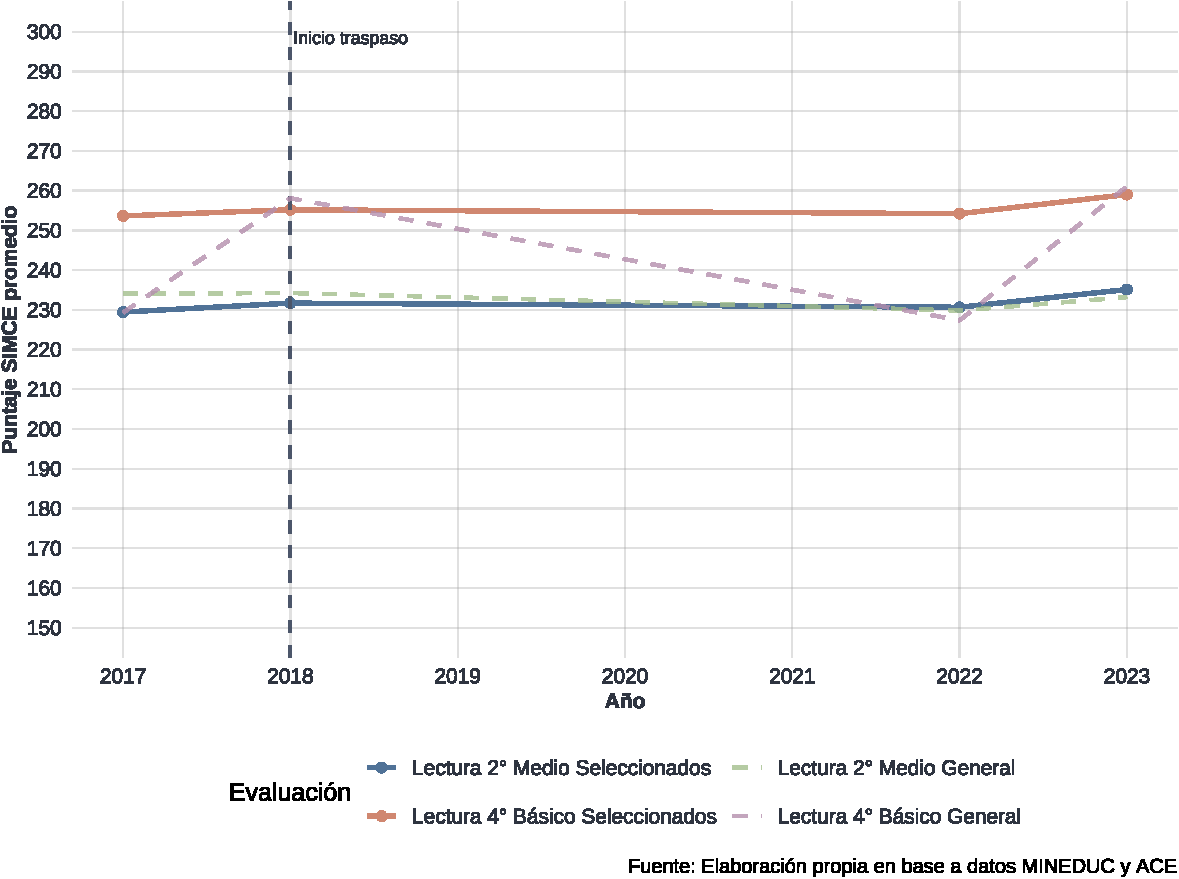
\includegraphics[width=0.8\linewidth,height=6in]{tesis_ver_final_files/figure-latex/grafico-simce-l-1} 

}

\caption{Evolución de puntajes SIMCE de Lectura (2017–2023)}\label{fig:grafico-simce-l}
\end{figure}

Como se puede observar, un gran obstáculo que se tiene a la hora de trabajar con esta dimensión es que durante los 2019 al 2021 no se encuentran bases de datos en la página web oficial de la ACE.
En particular, en los años 2020 y 2021 se cambió esta evaluación por un diagnóstico integral, voluntario de cada establecimiento, con motivo de la pandemia y el confinamiento que regía en el país (Diario Uchile, 2020).

A pesar de esto, se puede observar que los resultados no variaron mucho entre una edición a la otra en nuestros establecimientos.
Al último año disponible los puntajes han subido, aunque no mucho, en ambos niveles desde la primera observación.

\begin{figure}

{\centering 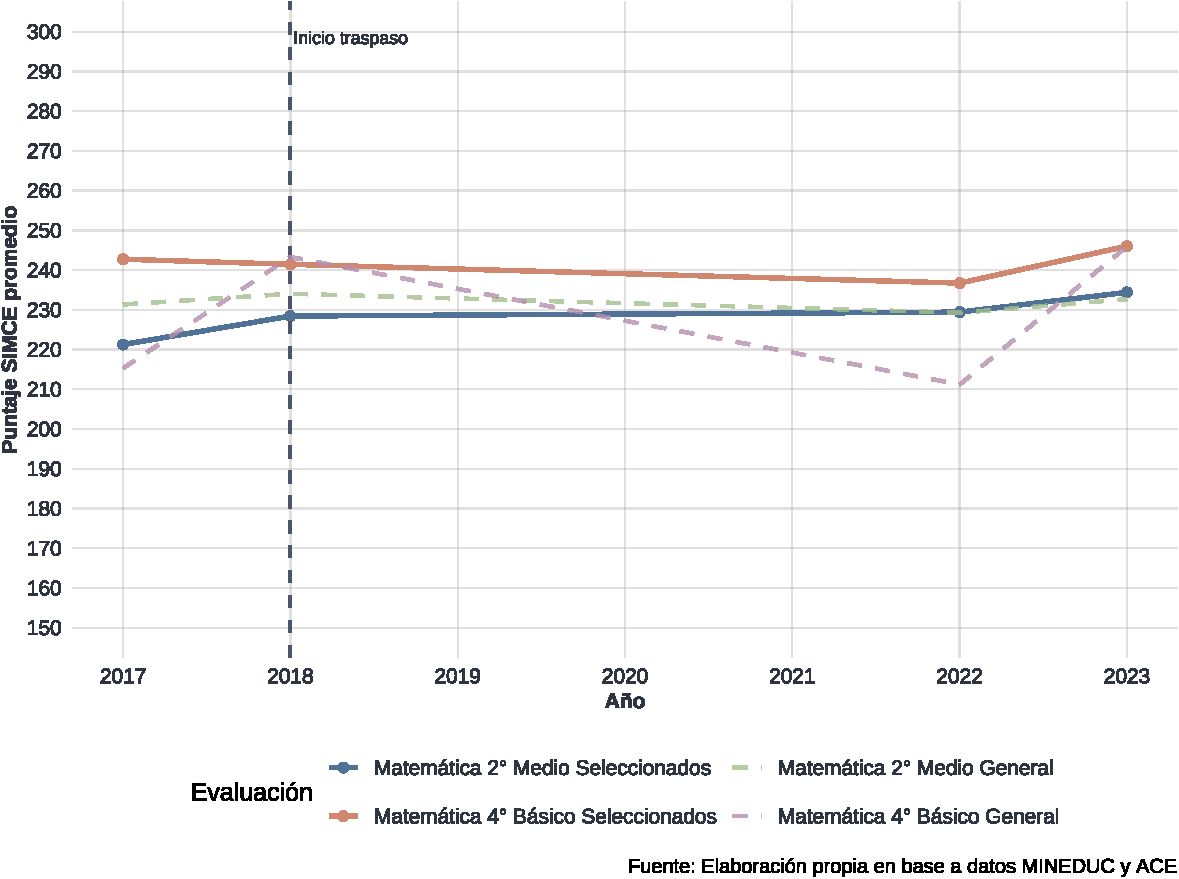
\includegraphics[width=0.8\linewidth,height=6in]{tesis_ver_final_files/figure-latex/grafico-simce-m-1} 

}

\caption{Evolución de puntajes SIMCE de Matemática (2017–2023)}\label{fig:grafico-simce-m}
\end{figure}

La situación cambia un poco cuando hablamos del SIMCE de matemáticas en el gráfico \ref{fig:grafico-simce-m}.
Aquí antes del traspaso los establecimientos se ubicaban bastante bajo el promedio general en ambos niveles, pero luego del traspaso, estas distancias han ido reduciéndose cada vez más, incluso superando el promedio para cuarto básico.
El nivel de segundo medio sigue la tónica del gráfico anterior ubicándose por debajo del promedio nacional, aunque durante 2022 a 2023 se observa un aumento de los puntajes, acercándose al nivel nacional.

En general, si comparamos ambos gráficos encontramos que la dimensión de puntaje SIMCE de lenguaje en los establecimientos que seleccionamos tiene un mejor desempeño que el de matemáticas, donde aún hay muchas brechas por cerrar.
Aunque siempre hay que tener en cuenta el contexto nacional durante los años en que no se rindió el SIMCE, que sin dudas afectó la capacidad de aprendizaje de los alumnos.
Cuestión que se observa con la baja generalizada de puntajes desde 2019 hasta 2022, tanto en nuestros establecimientos como en general.

\subsubsection{Ruralidad y matrícula}\label{ruralidad-y-matruxedcula}

En este apartado revisaremos las dimensiones de ruralidad, y luego de matrícula de alumnos en los SLEP que componen la muestra.

En primer lugar, nos referiremos a la ruralidad.
La figura \ref{fig:grafico-ruralidad} nos muestra la cantidad de establecimientos rurales y urbanos se encuentran en la muestra.

\begin{figure}

{\centering 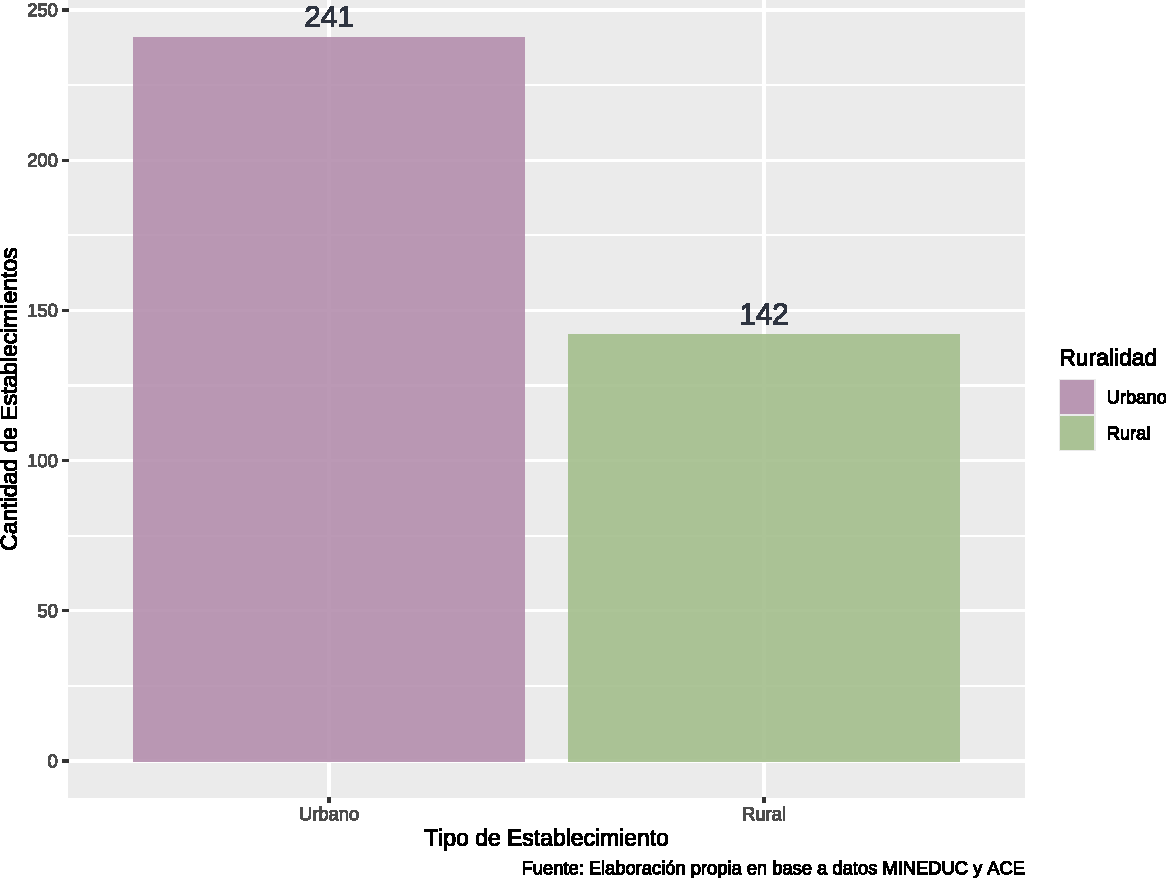
\includegraphics[width=0.8\linewidth,height=6in]{tesis_ver_final_files/figure-latex/grafico-ruralidad-1} 

}

\caption{Número de establecimientos rurales y urbanos}\label{fig:grafico-ruralidad}
\end{figure}

Vemos que la muestra contiene más establecimientos urbanos que rurales, aunque de igual manera se tiene una buena cantidad de establecimientos de tipo rural.
Resulta menester ver la distribución de estos por Servicio Local.

La tabla \ref{tab:tabla-ruralidad} contiene la información por SLEP de la cantidad de establecimientos que son urbanos o rurales: \newpage

\begin{table}[!h]
\centering
\caption{\label{tab:tabla-ruralidad}Establecimientos rurales y urbanos por SLEP}
\centering
\resizebox{\ifdim\width>\linewidth\linewidth\else\width\fi}{!}{
\begin{tabular}[t]{>{\raggedright\arraybackslash}p{3.8cm}>{\centering\arraybackslash}p{2.1cm}>{\centering\arraybackslash}p{2.1cm}>{\centering\arraybackslash}p{2.1cm}>{\centering\arraybackslash}p{2.1cm}>{\centering\arraybackslash}p{2.5cm}}
\toprule
SLEP & Urbano & \% Urbano & Rural & \% Rural & Total\\
\midrule
\textbf{\cellcolor{gray!10}{Andalién Sur}} & \cellcolor{gray!10}{45} & \cellcolor{gray!10}{66.2} & \cellcolor{gray!10}{23} & \cellcolor{gray!10}{33.8} & \cellcolor{gray!10}{68}\\
\textbf{Barrancas} & 50 & 94.3 & 3 & 5.7 & 53\\
\textbf{\cellcolor{gray!10}{Chinchorro}} & \cellcolor{gray!10}{30} & \cellcolor{gray!10}{50} & \cellcolor{gray!10}{30} & \cellcolor{gray!10}{50} & \cellcolor{gray!10}{60}\\
\textbf{Costa Araucanía} & 22 & 32.8 & 45 & 67.2 & 67\\
\textbf{\cellcolor{gray!10}{Gabriela Mistral}} & \cellcolor{gray!10}{34} & \cellcolor{gray!10}{100} & \cellcolor{gray!10}{0} & \cellcolor{gray!10}{0} & \cellcolor{gray!10}{34}\\
\addlinespace
\textbf{Huasco} & 27 & 50.9 & 26 & 49.1 & 53\\
\textbf{\cellcolor{gray!10}{Puerto Cordillera}} & \cellcolor{gray!10}{33} & \cellcolor{gray!10}{68.8} & \cellcolor{gray!10}{15} & \cellcolor{gray!10}{31.2} & \cellcolor{gray!10}{48}\\
\textbf{Total} & 241 & No aplica & 142 & No aplica & 383\\
\bottomrule
\multicolumn{6}{l}{\rule{0pt}{1em}Fuente: Elaboración propia en base a datos MINEDUC y ACE.}\\
\end{tabular}}
\end{table}

Como se puede observar, tenemos varias configuraciones de ruralidad, desde un SLEP 100\% urbano como lo es Gabriela Mistral de la Región Metropolitana, hasta otros con mayor proporción de establecimientos rurales como lo son el de Costa Araucanía o Huasco.
Esta información será de mucha utilidad más adelante en nuestra investigación.

La figura \ref{fig:grafico-matricula} muestra la evolución de la matrícula desde 2017 a 2024 en los establecimientos que componen la muestra.
Como se mencionó en el marco metodológico, tenemos una muestra de poco más de 100 mil alumnos en los 7 Servicios Locales.

\begin{figure}

{\centering 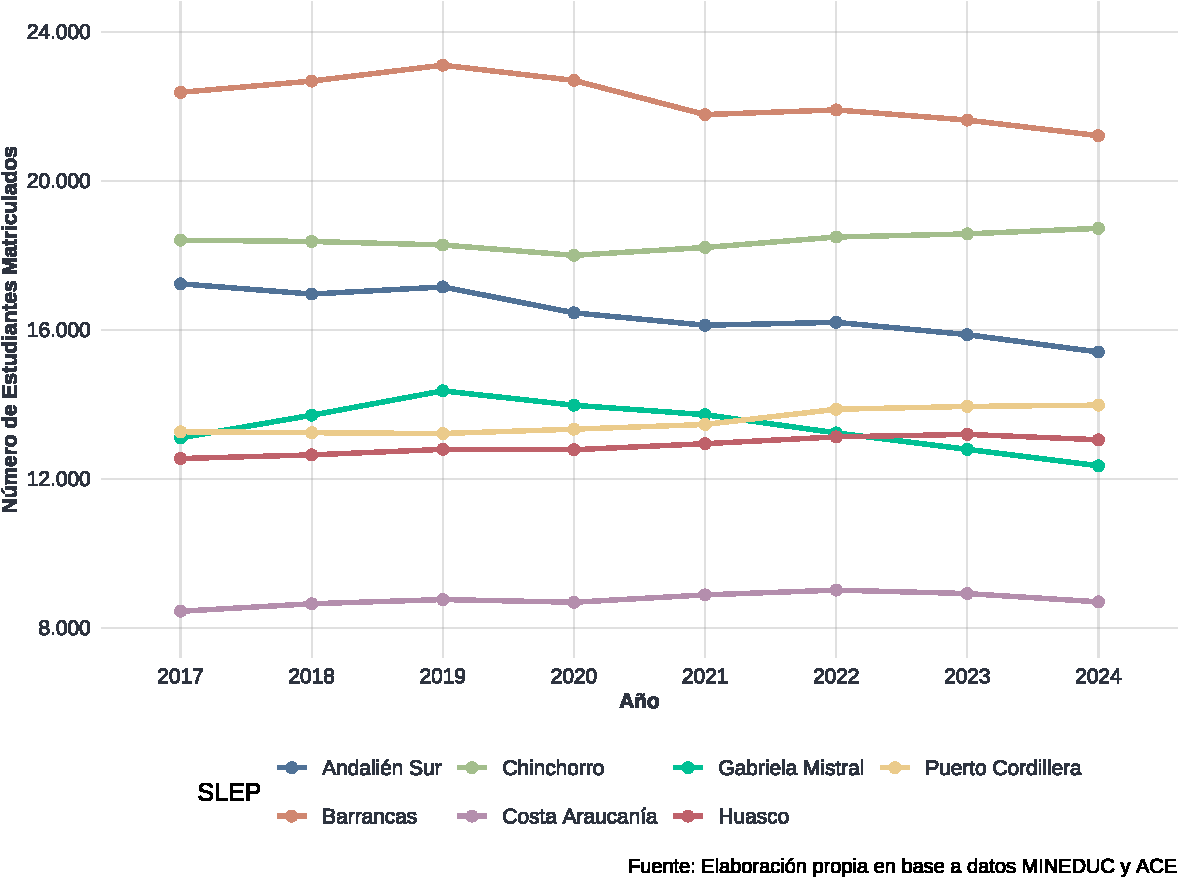
\includegraphics[width=0.8\linewidth,height=6in]{tesis_ver_final_files/figure-latex/grafico-matricula-1} 

}

\caption{Evolución de matrícula por SLEP}\label{fig:grafico-matricula}
\end{figure}

En los SLEP Chinchorro y Costa Araucanía se observa un leve aumento de los estudiantes respecto a la primera observación, mientras que Servicios Locales como el de Barrancas, Gabriela Mistral y Andalién Sur disminuyen una vez completado su traslado.
Los dos primeros mencionados comparten la característica de ser de la Región Metropolitana y contar con bajos niveles de ruralidad.
EL SLEP Andalién Sur, por su parte, también tiene más características urbanas que rurales, aunque en menor proporción que las dos primeras.

Si bien el tipo de establecimiento por SLEP no parece indicar una baja en la cantidad de matriculados, resulta llamativo ver que los SLEP Chinchorro y Costa Araucanía, los que tienen mayor índice de ruralidad, mantengan e incluso aumenten su matrícula respecto a la primera observación, mientras que los que mencionamos en el párrafo anterior la disminuyen.

\subsubsection{Docentes y asistentes}\label{docentes-y-asistentes}

Continuando con nuestro análisis, terminaremos el análisis descriptivo de los SLEP con las características de trabajadores de la educación, en las dimensiones de docentes y asistentes.

La figura \ref{fig:grafico-genero} muestra la proporción de género por SLEP, y como se observa la mayor parte de docentes son mujeres en los SLEP seleccionados, con diferencia, siendo más de la mitad en todos.
Esto es evidencia de una realidad que se conoce, de que la educación básica y media es un campo en el que mayoritariamente se desempeñan mujeres.

En esta misma línea, el gráfico \ref{fig:grafico-genero-horas} muestra la carga horaria por género, donde la distribución es bastante pareja, pero las mujeres tienden a tener contratos por más horas que los hombres (35,8 de los hombres y 38,1 de mujeres).

\begin{figure}

{\centering 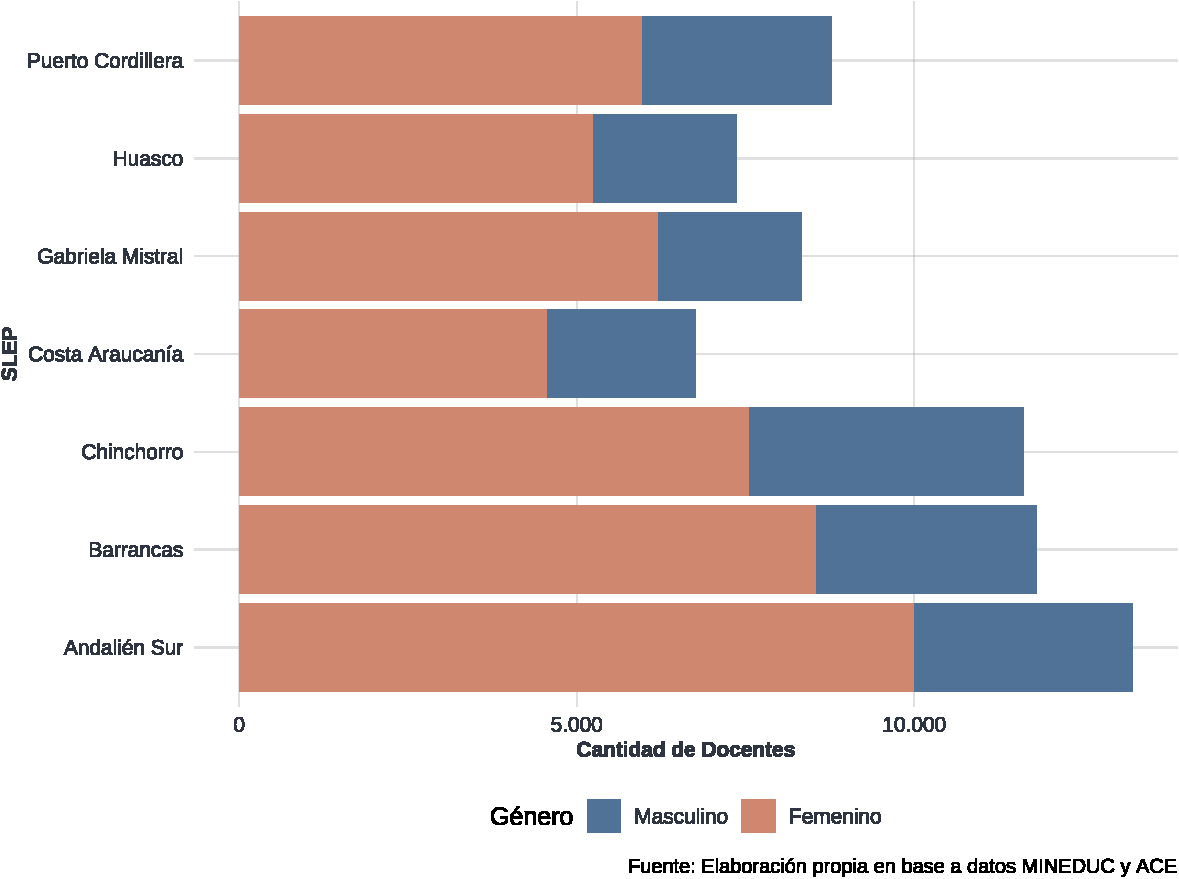
\includegraphics[width=0.8\linewidth,height=6in]{tesis_ver_final_files/figure-latex/grafico-genero-1} 

}

\caption{Proporción de género por docentes SLEP}\label{fig:grafico-genero}
\end{figure}

\begin{figure}

{\centering 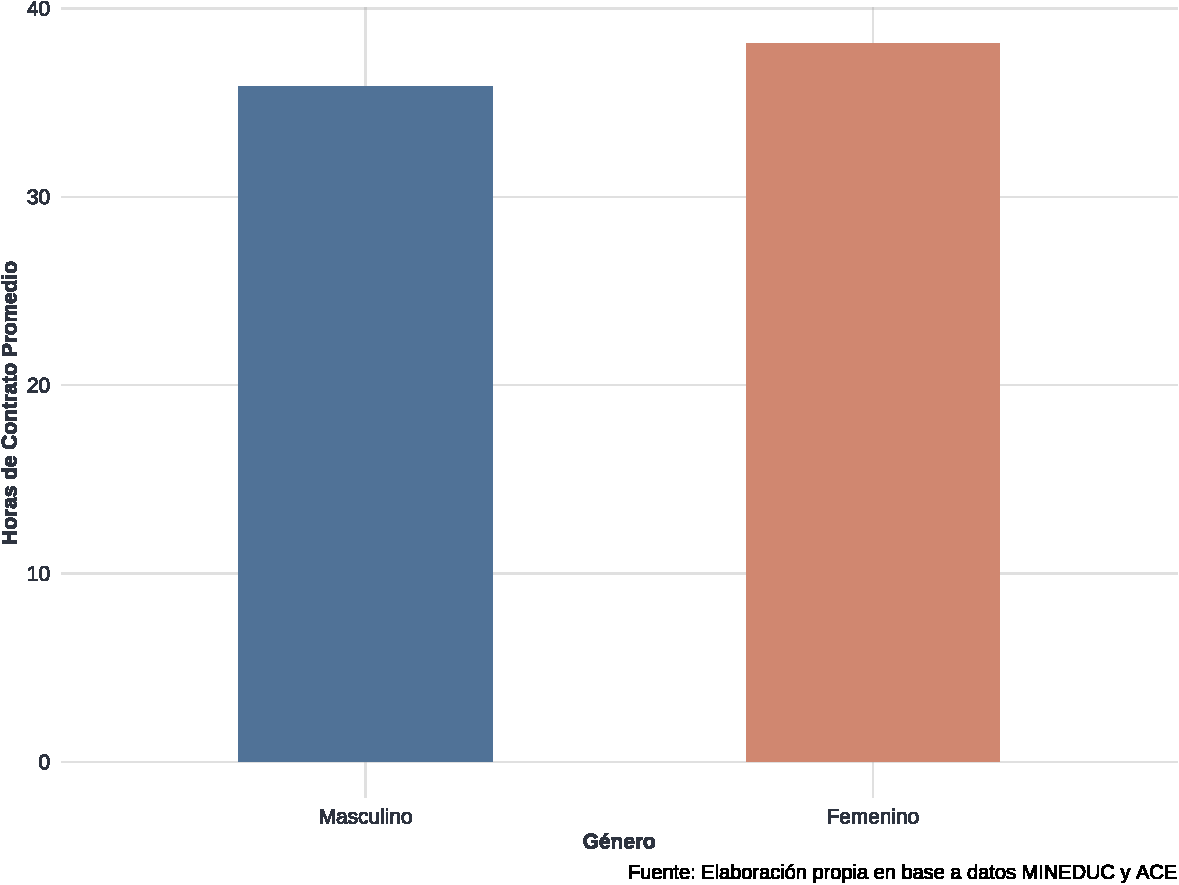
\includegraphics[width=0.8\linewidth,height=6in]{tesis_ver_final_files/figure-latex/grafico-genero-horas-1} 

}

\caption{Promedio de horas trabajadas por género}\label{fig:grafico-genero-horas}
\end{figure}

Para finalizar este apartado, se analizará brevemente la dimensión de asistentes de la educación, que son por lo general funcionarios que desempeñan tareas fundamentales dentro de los establecimientos, pero que no son docencia en aula.
Ejemplos de ellos son inspectores, trabajadores de aseo y ornato, asistentes profesionales y para docentes, entre otros.

La información principal que se usará de esta dimensión son las horas trabajadas totales por estamento, de 2017 a 2024, como se muestra en la figura \ref{fig:grafico-asistentes-jorn}, los para docentes son quienes concentran la mayor cantidad de tiempo trabajado en los establecimientos, luego los auxiliares y finalmente los asistentes profesionales.

Revisada la página web del MINEDUC, los para docentes se entienden de manera bastante amplia, ya que pueden ser desde administrativos hasta auxiliares de aseo (Ministerio de Educación, s.~f.).

\begin{figure}

{\centering 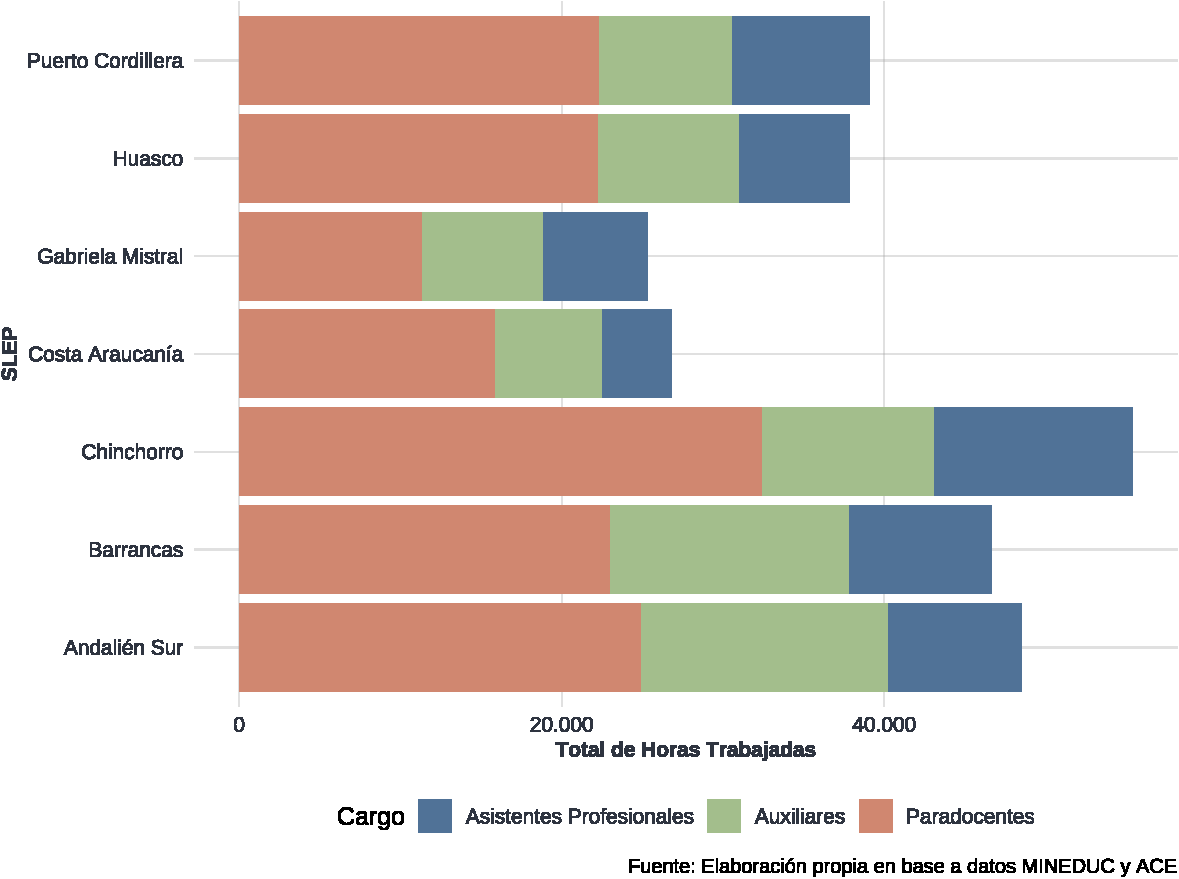
\includegraphics[width=0.8\linewidth,height=6in]{tesis_ver_final_files/figure-latex/grafico-asistentes-jorn-1} 

}

\caption{Carga horaria por estamento}\label{fig:grafico-asistentes-jorn}
\end{figure}

\subsection{Reducción de dimensionalidad con PCA y agrupamiento con K-Means}\label{reducciuxf3n-de-dimensionalidad-con-pca-y-agrupamiento-con-k-means}

Siguiendo al proceso necesario para reducir la dimensionalidad de los datos establecidos en la estrategia metodológica, se determinó el número apropiado de dimensiones a mantener, en base a la varianza explicada acumulada de cada componente.

Para ello, el conjunto de datos se filtró, eliminando columnas redundantes, estandarizó, para no tener problemas con las escalas, y se manejaron correctamente las variables categóricas, separándoles del conjunto que se usará, ya que son solamente identificaciones, como región, año, establecimiento, etc.
Luego de este proceso, nuestra base de datos que usaremos consta de 29 columnas que contienen la información que hemos esbozado hasta ahora.
El detalle de cada variable se puede consultar en el Anexo A.

Para nuestra investigación, consideramos que una tolerancia de 90\% de varianza explicada es prudente, lo cual como muestra el gráfico \ref{fig:grafico-var-acum} se logra con alrededor de 9 y 10 componentes.

\begin{figure}

{\centering 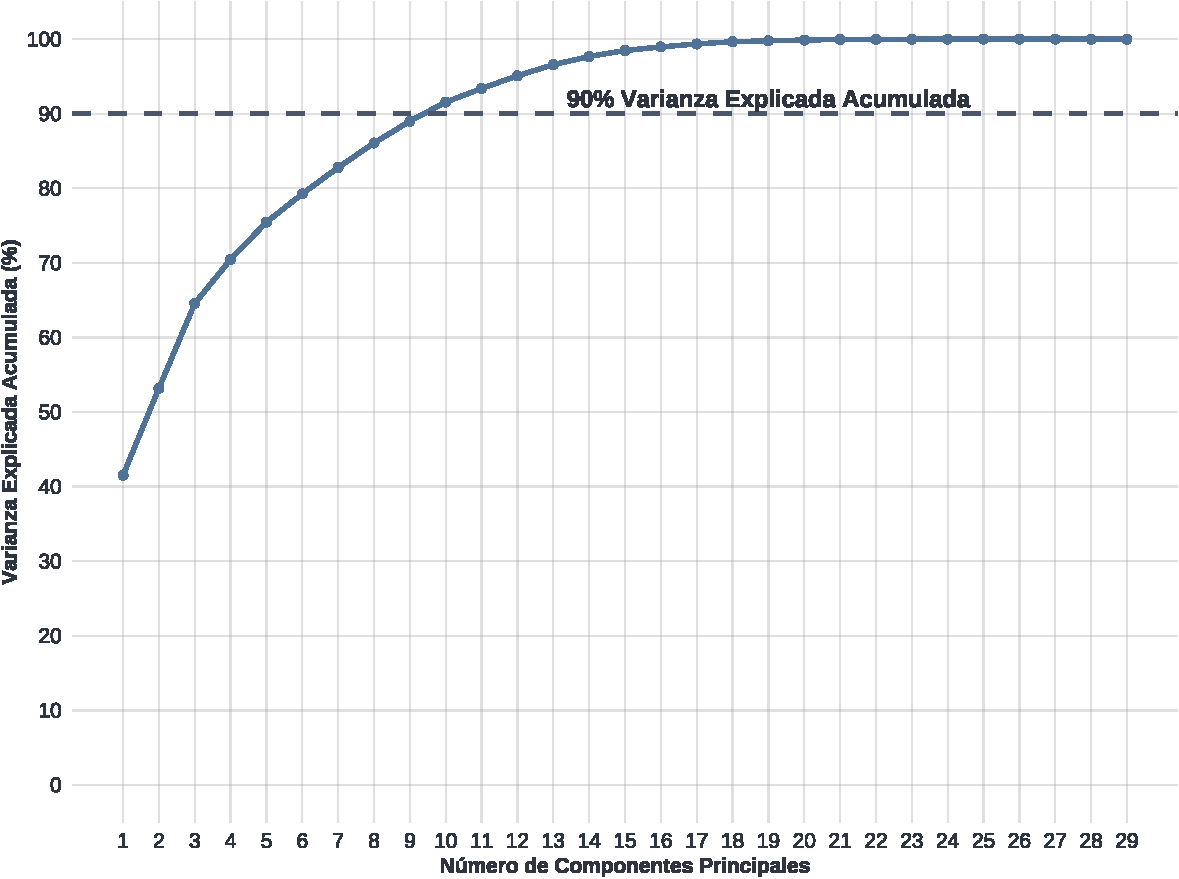
\includegraphics[width=0.8\linewidth,height=6in]{tesis_ver_final_files/figure-latex/grafico-var-acum-1} 

}

\caption{Varianza explicada acumulada en análisis de componentes principales (PCA)}\label{fig:grafico-var-acum}
\end{figure}

Para ver en detalle la contribución de cada variable para crear estos componentes principales, se puede consultar el Anexo B, en él se encuentra contenida información complementaria para comprender el proceso de creación de los dos primeros componentes principales que son cruciales.

Una vez elegida la cantidad de dimensiones reducidas que tendremos (en nuestro caso, 10), nuestro PCA está completo.
Ahora, viene la parte de elegir el número de centroides en los que se separará nuestro conjunto de datos, y para ello se usó, siguiendo la bibliografía consultada, el método del codo explicado en Umargono et~al. (2020) y también revisado en Gutierrez (2021).

Este método consiste en graficar la suma de los errores cuadráticos (SSE) para distintos valores de K y observar el punto donde la disminución comienza a desacelerarse de manera notoria, formando visualmente un ``codo''.
Ese punto representa un equilibrio entre la complejidad del modelo y la cohesión de los clústers, permitiendo seleccionar un número adecuado de agrupaciones sin sobreajustar el modelo.
En su estudio, Umargono et al.~demostraron que aplicar esta técnica no solo mejora la representatividad de los clústers obtenidos, sino que además reduce significativamente el número de iteraciones requeridas por el algoritmo, optimizando así el proceso de agrupamiento (Umargono et~al., 2020, pp. 127-129).

Como se ve en el gráfico \ref{fig:grafico-codo}, el codo se empieza a formar en 2 grupos y se mantiene así hasta 4 o 5 grupos.
Luego de eso, la ganancia de baja de los errores comienza a decaer, como es común en esta metodología.

\begin{figure}

{\centering 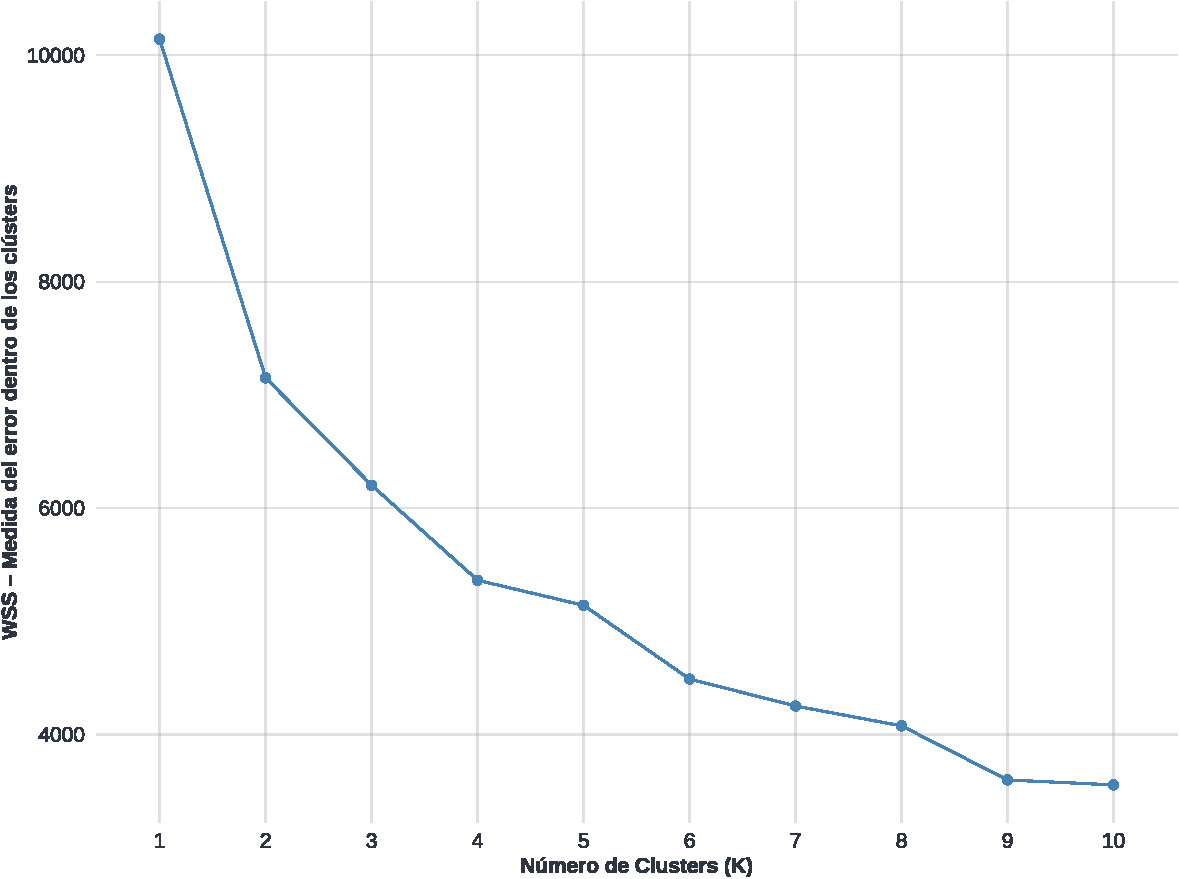
\includegraphics[width=0.8\linewidth,height=6in]{tesis_ver_final_files/figure-latex/grafico-codo-1} 

}

\caption{Método del codo para determinar número óptimo de clústers (K)}\label{fig:grafico-codo}
\end{figure}

En un proceso iterativo, se decidió entrenar distintas instancias de K-Means (de 2 a 10 centroides) para evaluar el desempeño de los \emph{clústers.} Para ello, se usó la métrica de el puntaje de silueta (\emph{silhouette score} en inglés).

Esta métrica analiza las distancias entre los \emph{clústers} generados para ver qué tan similares son intra-grupo y que tan diferentes son extra-grupo.
Su valor va desde -1 a 1, donde valores cercanos a -1 nos indica que el elemento está en el grupo equivocado, 0 nos dice que podría estar en cualquier otro (nuestro algoritmo no detectó diferencias o similitudes) y valores cercanos a 1 nos indica que el elemento está en el grupo correcto (Shahapure \& Nicholas, 2020).

Es importante mencionar que esta técnica de evaluación -al igual que la del codo- no es infalible, ya que la cantidad y calidad de clúster dependen más bien de nuestros objetivos y conjunto de datos, pero es una buena guía para ver que tan bien están siendo categorizados los datos.

Los resultados de dicho proceso iterativo se encuentran contenidos en la tabla \ref{tab:tabla-sil}.

\begin{table}[!h]
\centering
\caption{\label{tab:tabla-sil}Puntaje de silueta según número de clústers (K = 2 a 10)}
\centering
\resizebox{\ifdim\width>\linewidth\linewidth\else\width\fi}{!}{
\begin{tabular}[t]{>{\centering\arraybackslash}p{3cm}>{\centering\arraybackslash}p{3cm}}
\toprule
Número de clústers & Puntaje\\
\midrule
\textbf{\cellcolor{gray!10}{2}} & \cellcolor{gray!10}{0.29}\\
\textbf{3} & 0.20\\
\textbf{\cellcolor{gray!10}{4}} & \cellcolor{gray!10}{0.23}\\
\textbf{5} & 0.23\\
\textbf{\cellcolor{gray!10}{6}} & \cellcolor{gray!10}{0.23}\\
\addlinespace
\textbf{7} & 0.20\\
\textbf{\cellcolor{gray!10}{8}} & \cellcolor{gray!10}{0.22}\\
\textbf{9} & 0.23\\
\textbf{\cellcolor{gray!10}{10}} & \cellcolor{gray!10}{0.22}\\
\bottomrule
\end{tabular}}
\end{table}

Vemos que nuestro algoritmo, con 10 dimensiones, varía desde 0,29 en 2 grupos y 0,20 en 7 grupos, teniendo resultados bastante homogéneos durante todas las pruebas.
En base a lo anterior, y complementando con el método del codo, nos quedaremos con 3 grupos, ya que a pesar de no tener el mejor puntaje de silueta, esta diferencia es mínima.
Otra razón es que el hecho de tener dos grupos simplifica de sobremanera el análisis.

Los resultados de silueta por grupo se encuentran en el Anexo D, donde se puede consultar en detalle el puntaje y comportamiento de cada grupo utilizando esta puntuación.

\subsection{Resultados de agrupamiento}\label{resultados-de-agrupamiento}

Para finalizar este apartado, en la figura \ref{fig:grafico-cluster} se muestran los 3 grupos generados por el algoritmo.
De manera preliminar, y meramente visualizando el gráfico, se puede observar que en general existe una separación heterogénea de los grupos, teniendo solapamiento respecto al grupo 1 que parece ser el que presenta un desafío mayor al algoritmo.
A su vez, este grupo es el más numeroso.

\begin{figure}

{\centering 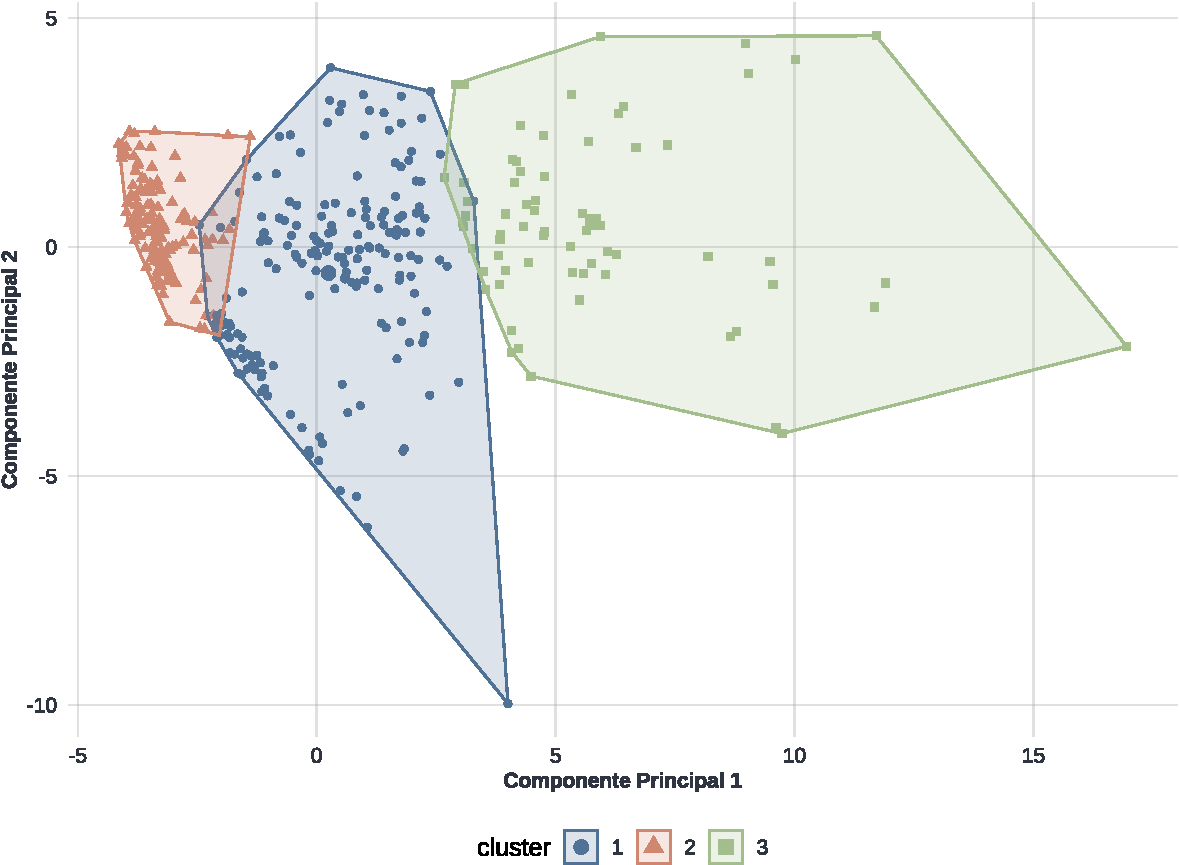
\includegraphics[width=0.8\linewidth,height=6in]{tesis_ver_final_files/figure-latex/grafico-cluster-1} 

}

\caption{Distribución de clústers identificados mediante K-Means y PCA}\label{fig:grafico-cluster}
\end{figure}

El detalle de Servicios Locales por grupo se encuentra en el gráfico \ref{fig:grafico-detalle-cluster}.
Como se observa, el único Servicio Local que se categorizó fuertemente fue el de Costa Araucanía, y en el resto de los grupos, con mayor o menor medida, se encuentran establecimientos de todos los SLEP.

\begin{figure}

{\centering 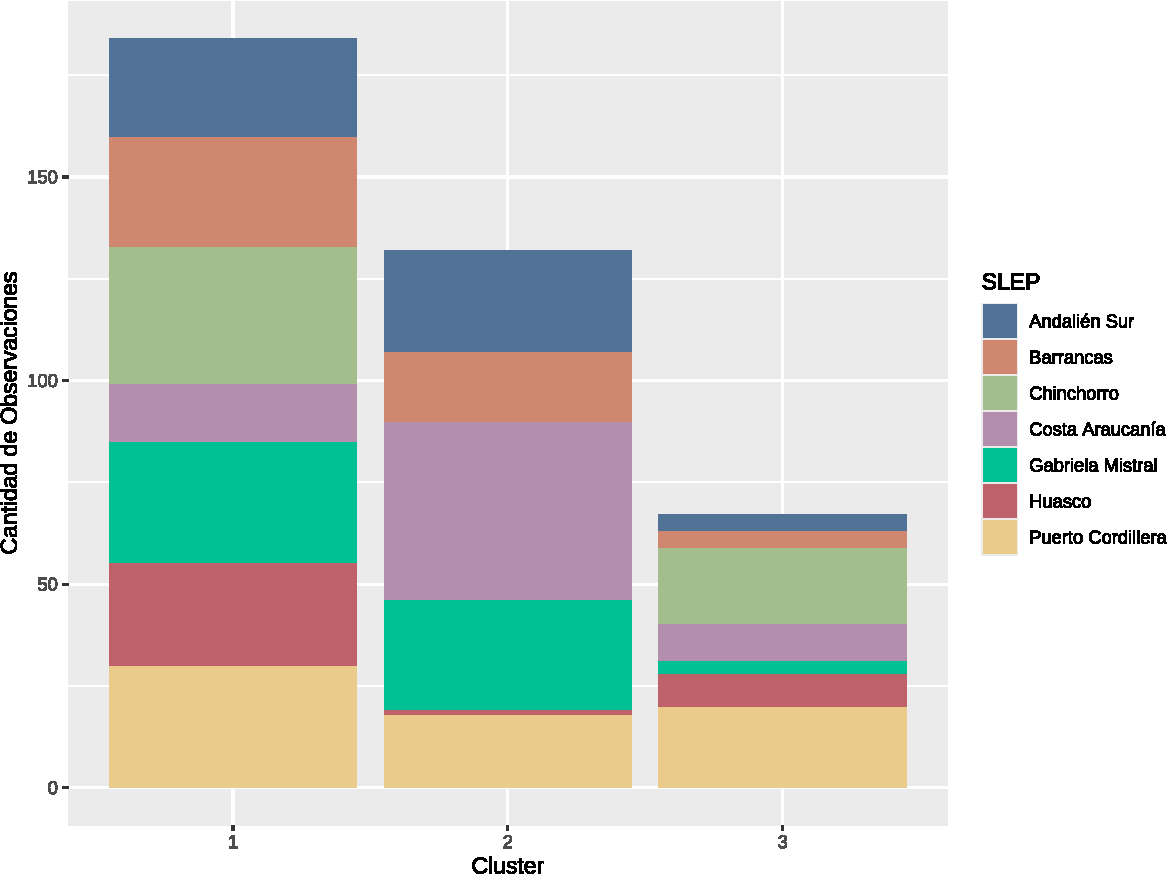
\includegraphics[width=0.8\linewidth,height=6in]{tesis_ver_final_files/figure-latex/grafico-detalle-cluster-1} 

}

\caption{Cantidad de SLEP por clúster}\label{fig:grafico-detalle-cluster}
\end{figure}

Finalmente, el detalle de las características principales de los grupos en relación con las dimensiones trabajadas se encuentran contenidas en el gráfico \ref{fig:grafico-caract-cluster}, este gráfico simplifica un poco los resultados obtenidos para cada grupo mediante una normalización, donde valores cercanos a 0 y de color azul representan menores puntuaciones en la variable, y valores cercanos a 1 y de color naranja representa mayor concentración de esa variable.

Se puede observar que los grupos son totalmente distintos, y variables como las referidas a los alumnos prioritarios, horas de aula y matrícula parecen ser las principales que separan los grupos uno de otro.
Estas características serán detalladas en el apartado de discusión y conclusiones.

Para mayor información respecto a las variables y su rol dentro de cada grupo, el Anexo C presenta información complementaria respecto a qué tanto pondera cada variable en cada grupo.

\begin{figure}

{\centering 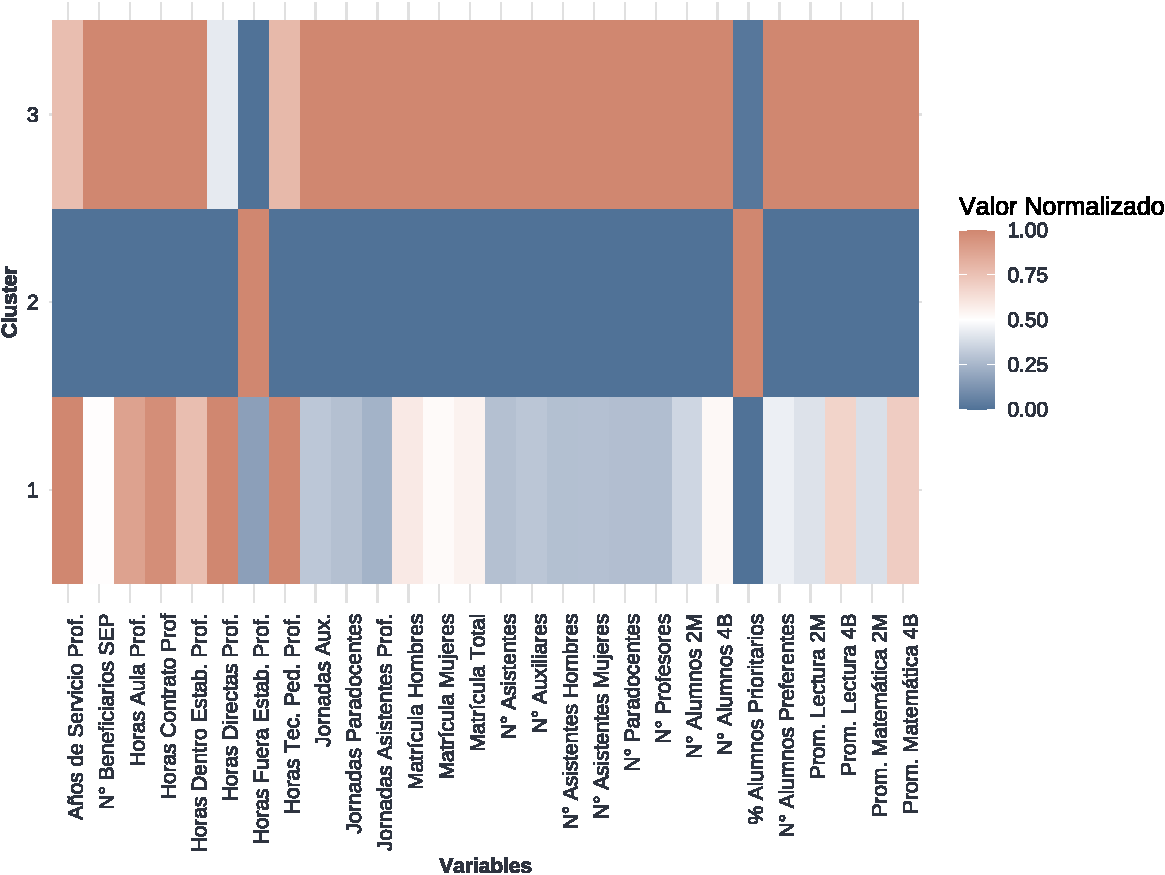
\includegraphics[width=0.8\linewidth,height=6in]{tesis_ver_final_files/figure-latex/grafico-caract-cluster-1} 

}

\caption{Mapa de calor de variables normalizadas por clúster}\label{fig:grafico-caract-cluster}
\end{figure}

\newpage

\section{Discusión}\label{discusiuxf3n}

El análisis de datos cuantitativos para darnos una mirada acerca de los SLEP se relaciona directamente con los conceptos que vimos en las inspiraciones teóricas para el fundamento de esta investigación en 3 principales ejes:

\subsection{Capital humano y datos generales de establecimientos}\label{capital-humano-y-datos-generales-de-establecimientos}

Directamente relacionada con el enfoque del capital humano, al analizar los datos generales de los colegios nos damos cuenta de la disparidad que existe entre regiones de nuestro país.
La ruralidad sigue siendo un gran desafío para lograr buenos resultados académicos y atraer a docentes y asistentes de educación.
Los SLEP con mayor tendencia a la ruralidad suelen tener un cuerpo académico más acotado, así como también menor cantidad de alumnos, pero esto también se puede traducir en menores resultados académicos y asignación de recursos, así como mayor carga laboral para el cuerpo administrativo y docente de estos, como se vio reflejado en el \ref{fig:grafico-asistentes-jorn}, donde estos establecimientos superaban en horas de trabajo a SLEP más urbanos como el Gabriela Mistral o Barrancas.

Si bien esto no es uniforme, es un hallazgo importante para la toma de decisiones respecto a cómo administrar estos establecimientos

En esta misma línea, cuando hablamos de cómo se distribuyen las tareas en función de género, se hace importante observar gráficos como los \ref{fig:grafico-genero} y \ref{fig:grafico-genero-horas}.
Si bien el objetivo de esta investigación no es analizar estos datos con perspectiva de género, es una buena dimensión para explorar, con análisis de corte cualitativo y cuantitativo.

Un enfoque de este estilo podría dilucidar por qué existen diferencias tan significativas en el número de hombres y mujeres que trabajan en los establecimientos seleccionados, y también, por qué a pesar de ello son las mujeres docentes quienes figuran con horas formales de contrato mayores.
A su vez, se podrían incluir dimensiones como las remuneraciones docentes para ver cómo se comporta esta variable en relación con lo anterior.

Finalmente, al analizar los resultados SIMCE de los establecimientos, se deduce que estos no están tan atrás comparados a los resultados generales, siendo ligeramente inferiores en la última vez que se rindió esta prueba, pero durante 2022 los alumnos de cuarto básico estuvieron sobre el promedio nacional.

Es importante mencionar que con la poca cantidad de años que se graficaron antes del traspaso, y también con la no rendición de las pruebas durante 2019 a 2021, esta arista no aporta tanto al análisis realizado, pero es interesante ver que, a pesar del traspaso de funciones de la municipalidad al Servicio Local, los puntajes no han tenido mayores variaciones.
Esto nos habla de lo importante que es el colegio como institución y como este se administra a nivel micro (dentro del establecimiento).

\subsection{El traspaso de funciones administrativas y su vinculación con los datos estudiados}\label{el-traspaso-de-funciones-administrativas-y-su-vinculaciuxf3n-con-los-datos-estudiados}

Como fue esbozado en el párrafo anterior, el traspaso de funciones administrativas no parece tener mayor relación en cómo se están comportando los establecimientos, aunque esto puede ser también por la poca temporalidad disponible para estudiar a los mismos.
También siempre es importante lo anómalos que fueron los años 2020, 2021 e incluso 2022, donde la pandemia rompió con toda normalidad lo que se venía haciendo cuando los establecimientos dependían de la municipalidad o corporación.

A pesar de todo, esta dimensión fue importante para entender cómo se configura actualmente un Servicio Local y saber también de qué manera se administra.
El impacto que pueda tener la nueva administración se podrá medir con el tiempo y con análisis de tipo cualitativo o mixto, ya que las dimensiones publicadas por el MINEDUC que fueron elegidas para investigación no dicen mucho acerca de esto.

\subsection{La ciencia de datos y la toma de decisiones basada en datos}\label{la-ciencia-de-datos-y-la-toma-de-decisiones-basada-en-datos}

Este apartado es aquel que da mayor sustento a la discusión de los resultados que se obtuvieron al realizar esta investigación, y que fue la base para responder la pregunta de investigación.

El hecho de tener datos tan variados que vienen desde el MINEDUC respecto a los establecimientos en general hace necesaria su visualización para que no se queden siendo solamente eso, números.
El esfuerzo de esta investigación se encuentra en darles sentido y poder tomar decisiones respecto a los datos empíricos, usando para ello gráficos clásicos como también procesamiento de datos avanzado, teniendo siempre presente lo poderosas que son las herramientas de machine learning y sus derivados para lograr llegar a buen puerto con el procesamiento de información.

Este apartado es fundamental para la administración pública en la actualidad, ya que siempre se pondrá en tela de juicio la capacidad de gestionar tantos servicios por parte del Estado, y no solamente es necesaria más información sino que mejor manera de comunicarla tanto internamente como a la ciudadanía.
El uso de herramientas avanzadas es un primer paso hacia una modernización de prácticas y manejo de datos dentro del Estado, que puede mejorar la eficiencia y el cumplimiento de objetivos en el área de educación como en cualquier otra que sea de interés público.

Esta investigación da luces sobre las características de los SLEP seleccionados para focalizar las medidas de inversión o de capital humano en las dimensiones donde los grupos están bajo otros, o reforzar lo que se viene haciendo bien.
También, a futuro, nos permite hacer comparaciones entre el momento actual con el futuro.
Se pueden establecer pautas de acción dentro de los Servicios Locales pero también dentro de los colegios.

Si bien el uso de herramientas tecnológicas de procesamiento de datos como los métodos vistos en esta investigación es de gran ayuda para lograr lo anterior, siempre existe espacio para mejora.
Como se observó en el gráfico de clústers, los grupos no están tan definidos, para lograr una selección más robusta y evitar caer en sesgos, se tendrían que usar algoritmos más avanzados que puedan mezclar datos categóricos y numéricos sin confundirlos, reducir el número de variables o agregar o quitar dimensiones.
A pesar de todo, los resultados son aceptables y dieron cumplimiento a lo planteado en la elaboración de la estrategia metodológica, objetivos y pregunta.

Creo que esta investigación se podría nutrir de mejor manera si se tuvieran más intervalos de años y más dimensiones respecto a las características presupuestarias de los establecimientos, aunque lamentablemente las bases de datos disponibles al respecto no pudieron ser procesadas de la misma manera que las otras que aquí se vieron.

También, se podría procesar más información respecto a la zona geográfica de cada establecimiento y su vinculación con los SLEP y resultados.
Aquí se esbozó un poco con la ruralidad de los establecimientos seleccionados, pero un análisis de tipo territorial con mapas de comunas y regiones podría ser de mejor ayuda para que la administración local de cada SLEP pueda tener panoramas respecto a sus establecimientos.
Es una arista que se puede agregar en investigaciones un poco más acotadas a un solo SLEP, o a su conjunto de comunas y región.

Después de todo lo que se desarrolló en el apartado de resultados, creo que los objetivos se cumplieron a cabalidad, ya que como nos dicen los gráficos referentes a los grupos, se pueden establecer similitudes dentro de los grupos y se analizaron los datos provenientes de los establecimientos en la temporalidad definida.
Tanto la caracterización como el detalle de los cumplimientos de la hoja de ruta se presentarán en el siguiente apartado.

\newpage

\section{Conclusiones}\label{conclusiones}

El proceso anterior de investigación y muestra de resultados nos permitió generar una gran cantidad de información respecto a la muestra seleccionada en una primera instancia, y luego facilitó el agrupamiento de los establecimientos en grupos distintos entre ellos.
Esto tiene concordancia con nuestros objetivos, pregunta de investigación y estrategia metodológica.

La limpieza, procesamiento y transformación de los datos en información no trivial en esta investigación se expresa en la caracterización de cada grupo que obtuvimos en la figura \ref{fig:grafico-cluster}, y es esta la respuesta a la pregunta de investigación que nos planteamos al principio.

Los SLEP seleccionados se pueden agrupar de 3 maneras distintas, y las características de cada grupo son:

\textbf{Grupo 1: establecimientos intermedios y equilibrados}

Este grupo presenta niveles medios en la mayoría de las variables.
Los establecimientos aquí no destacan por sobrecarga ni por bajos recursos, pero muestran una menor presencia de estudiantes prioritarios y preferentes en comparación con el grupo 2.

Las horas docentes son relativamente altas, y el rendimiento SIMCE se ubica entre los valores medios y altos, especialmente en Lectura.
Este grupo podría representar escuelas con una carga moderada y cierta eficacia educativa, operando en contextos mixtos en términos de vulnerabilidad.

Es el grupo que contiene mayor cantidad de Servicios Locales, con casi la mitad del total.

\textbf{Grupo 2: establecimientos de alta vulnerabilidad socioeconómica y ruralidad}

Este grupo concentra la mayor cantidad de estudiantes prioritarios, preferentes y beneficiarios de SEP.
Sin embargo, es el que muestra los niveles más bajos de matrícula total, personal asistente, auxiliares y para-docentes.
Además, presenta la menor carga horaria docente y el rendimiento SIMCE más bajo en todas las áreas.
Esto indica un escenario de alta vulnerabilidad y limitados recursos humanos, lo que puede afectar negativamente los resultados académicos.

Representa a escuelas con gran carga social y desafíos estructurales relevantes.
En este grupo es donde se ubica la mayor cantidad de establecimientos de tipo rural y pertenecientes al SLEP Costa Araucanía.

\textbf{Grupo 3: establecimientos con alto rendimiento académico y menor vulnerabilidad}

Este grupo destaca por obtener los puntajes más altos en todas las pruebas SIMCE, tanto en cuarto básico como segundo medio.

Tiene las cargas horarias docentes más altas, tanto dentro como fuera del establecimiento, junto con niveles elevados de matrícula y personal asistente.
A diferencia del grupo 2, aquí se observa una menor proporción de estudiantes prioritarios, preferentes o beneficiarios de SEP.

Es un grupo con menor carga social y alta exigencia profesional, lo que sugiere un entorno más estable y con condiciones favorables para el aprendizaje.
A su vez, es el grupo con menor cantidad de SLEP y donde se ubican los establecimientos pertenecientes a Servicios Locales con mayor porcentaje de colegios de tipo urbano.

La tabla \ref{tab:tabla-cluster-resumido} contiene una breve reseña de la información contenida en los párrafos anteriores, de manera de hacer más comprensible su entendimiento.

\begin{table}[!h]
\centering
\caption{\label{tab:tabla-cluster-resumido}Características resumidas de cada grupo}
\centering
\resizebox{\ifdim\width>\linewidth\linewidth\else\width\fi}{!}{
\begin{tabular}[t]{>{\centering\arraybackslash}p{2cm}>{\raggedright\arraybackslash}p{10cm}}
\toprule
Grupo & Descripción\\
\midrule
\textbf{\cellcolor{gray!10}{1}} & \cellcolor{gray!10}{Escuelas con condiciones intermedias, carga docente moderada y equilibrio general. Presentan niveles medios de estudiantes prioritarios, preferentes y beneficiarios SEP. Contienen la mayor cantidad de SLEP.}\\
\textbf{2} & Escuelas con alta vulnerabilidad: concentran el mayor porcentaje de estudiantes prioritarios, preferentes y beneficiarios SEP. Tienen menor dotación de personal y los rendimientos académicos más bajos. Predominan los establecimientos rurales.\\
\textbf{\cellcolor{gray!10}{3}} & \cellcolor{gray!10}{Escuelas con alto rendimiento SIMCE y menores niveles de estudiantes prioritarios, preferentes y SEP. Presentan mayores cargas docentes y dotación profesional, en contextos más urbanos y estables.}\\
\bottomrule
\end{tabular}}
\end{table}

Ahora exploraremos el cumplimiento de los objetivos de investigación.

Con respecto al cumplimiento del objetivo principal, vemos que se cumplió de buena manera, durante la primera etapa de representación visual de datos.
Se encontraron las diferencias y similitudes en los gráficos que se mostraron en el apartado de resultados y que fueron analizados en la discusión de estos.
Aun así, se podría tener un mejor entendimiento del apartado de comparación pre y pos SLEP, pero los datos anteriores a 2017 disponibles son difíciles de trabajar, y para ser usados se debería tener otros enfoques de investigación que escapan a este trabajo.

Los objetivos específicos, por otro lado, fueron cubiertos a cabalidad, gracias a la combinación de PCA con K-Means.
Se pudieron generar los grupos y luego diferenciarlos en una primera instancia, para luego ser presentados en el apartado anterior sobre respuesta a la pregunta de investigación.

Lo anterior nos permite aprobar o descartar nuestras hipótesis:

\begin{itemize}
\item
  H1: Se rechaza esta hipótesis, los datos generales y de rendimiento que fueron graficados y analizados no sufrieron cambios tan bruscos luego del traspaso.
\item
  H2: Se acepta esta hipótesis, ya que sí existe cierta tendencia dentro de los grupos para tener representantes de uno u otro SLEP.
  Además, el hecho de que se encuentren establecimientos de todos los SLEP en todos los grupos da cuenta de lo heterogénea que es su composición
\item
  H3: Se acepta esta hipótesis, ya que como se mencionó en el apartado de resultados y discusión, los SLEP con alta tendencia a la ruralidad cuentan con menores trabajadores de la educación, así como también tienen tendencia a una menor matrícula y resultados académicos en las pruebas SIMCE de lectura y matemática en cuarto básico y segundo medio.
\end{itemize}

Este informe busca ser un insumo útil para comprender el estado actual de los establecimientos educacionales públicos, los Servicios Locales y el proceso de implementación de la Nueva Educación Pública en Chile.
A través del uso de herramientas de machine learning, se intentó abordar el problema con una perspectiva analítica que permitiera identificar patrones y caracterizar realidades diversas dentro del sistema.

Los gráficos generados permiten visualizar esta complejidad y entregan una mirada concreta sobre cómo han evolucionado los establecimientos tras el traspaso desde la administración municipal hacia los SLEP.
La disposición de esta información en un formato visual no solo busca facilitar la comprensión de grandes volúmenes de datos, sino también fomentar nuevas preguntas e interpretaciones por parte de quienes se aproximen a este estudio desde distintos enfoques.

En síntesis, esta investigación pretende aportar al fortalecimiento de la gestión y al uso más eficiente de los recursos humanos y económicos en esta nueva etapa de la educación pública.

A partir de los hallazgos presentados, se recomienda que futuras investigaciones profundicen en tres líneas:

\begin{enumerate}
\def\labelenumi{\arabic{enumi}.}
\item
  Evaluaciones que sigan la trayectoria de los SLEP en el tiempo y midan su impacto sostenido en los resultados educativos.
\item
  Estudios cualitativos territoriales que recojan percepciones de actores locales, como docentes y directivos, respecto a los cambios administrativos y pedagógicos a medida que más establecimientos den cumplimiento al traspaso dispuesto en la ley.
\item
  Análisis comparativos internacionales que permitan situar el caso chileno dentro de experiencias similares de transferencia de funciones en la administración de los establecimientos de la educación pública.
\end{enumerate}

Estas líneas permitirán seguir construyendo evidencia para mejorar las políticas públicas en educación y, con ello, avanzar hacia un sistema educativo más justo e igualitario.

\newpage

\section{Referencias}\label{referencias}

\phantomsection\label{refs}
\begin{CSLReferences}{1}{0}
\bibitem[\citeproctext]{ref-agencia_de_la_calidad_de_la_educacion_bases_nodate}
Agencia de la Calidad de la Educación. (s.~f.). \emph{Bases de {Datos}}. Recuperado 3 de abril de 2025, de \url{https://informacionestadistica.agenciaeducacion.cl/\#/bases}

\bibitem[\citeproctext]{ref-aurelien_geron_hands-machine_2017}
Aurélien Géron. (2017). \emph{Hands-{On} {Machine} {Learning} with {Scikit}-{Learn} \& {TensorFlow}} (4.ª ed.). O'Reilly Media, Inc.

\bibitem[\citeproctext]{ref-baleriola_traduccion_2021}
Baleriola, E., Contreras-Villalobos, T., \& Ramírez-Casas Del Valle, L. (2021). Traducción de la política educativa. {El} caso de la {Nueva} {Educación} {Pública}. \emph{Athenea Digital. Revista de pensamiento e investigación social}, \emph{21}(2). \url{https://doi.org/10.5565/rev/athenea.2910}

\bibitem[\citeproctext]{ref-barrientes_seborga_educacion_2020}
Barrientes Seborga, C. I. (2020). Educación. bien público impuro que promueve el crecimiento económico inclusivo. \emph{Revista Investigación y Negocios}, \emph{13}(21), 122-131. \url{http://www.scielo.org.bo/scielo.php?script=sci_abstract&pid=S2521-27372020000100011&lng=es&nrm=iso&tlng=es}

\bibitem[\citeproctext]{ref-bellei_nueva_2018}
Bellei, Cristián. (2018). \emph{Nueva educación pública: contexto, contenidos y perspectivas de la desmunicipalización} (1era. edición: noviembre de 2018). CIAE Centro de Investigación Avanzada en Educación, Universidad de Chile.

\bibitem[\citeproctext]{ref-bellei_ecos_2010}
Bellei, Cristián., Contreras, D., \& Valenzuela, J. P. (2010). \emph{Ecos de la revolución pingüina: avances, debates y silencios en la reforma educacional}. Universidad de Chile.

\bibitem[\citeproctext]{ref-berkowitz_servicios_2024}
Berkowitz, D., Araneda, S., Nuñez, D., Tham, M., Figueroa, I., Toro, V., Pérez, J., García, G., Videla, M., Beck, G., González, C., \& Espinosa, P. (2024). \emph{Servicios {Locales} de {Educación} {Pública} en {Números}: {Indicadores} educativos de servicios en régimen a 2023.} \url{http://bibliotecadigital.mineduc.cl//handle/20.500.12365/20253}

\bibitem[\citeproctext]{ref-biblioteca_del_congreso_nacional_de_chile_ley_2017}
Biblioteca del Congreso Nacional de Chile. (2017). Ley 21040. En \emph{Ley Chile}. \url{https://www.bcn.cl/leychile/navegar?idNorma=1111237}

\bibitem[\citeproctext]{ref-centro_de_estudios_mineduc_datos_nodate}
Centro de Estudios MINEDUC. (s.~f.). \emph{Datos {Abiertos}}. Recuperado 3 de abril de 2025, de \url{https://datosabiertos.mineduc.cl/}

\bibitem[\citeproctext]{ref-diario_uchile_pruebe_2020}
Diario Uchile. (2020). Pruebe {Simce} 2020 será reemplazada por una evaluación de carácter muestral y voluntaria. En \emph{Diario U de Chile}. \url{https://radio.uchile.cl/2020/06/17/pruebe-simce-2020-sera-reemplazada-por-una-evaluacion-de-caracter-muestral-y-voluntaria/}

\bibitem[\citeproctext]{ref-fayyad_data_1996}
Fayyad, U., Piatetsky-Shapiro, G., \& Smyth, P. (1996). From {Data} {Mining} to {Knowledge} {Discovery} in {Databases}. \emph{AI Magazine}, \emph{17}(3), 37-37. \url{https://doi.org/10.1609/aimag.v17i3.1230}

\bibitem[\citeproctext]{ref-fundacion_horizonte_ciudadano_herramientas_2024}
Fundación Horizonte Ciudadano. (2024). \emph{Herramientas para aportar a la {Nueva} {Educación} {Pública} desde los municipios}. \url{https://rumbocolectivo.cl/wp-content/uploads/2025/01/Herramientas-para-aportar-a-la-Nueva-Educacion-Publica-desde-los-municipios.pdf}

\bibitem[\citeproctext]{ref-garcia-gonzalez_knowledge_2019_a}
García-González, J. R., Sánchez-Sánchez, P. A., Orozco, M., \& Obredor, S. (2019). Knowledge {Capture} for the {Prediction} and {Analysis} of {Results} of the {Quality} {Test} of {Higher} {Education} in {Colombia}. \emph{Formación universitaria}, \emph{12}(4), 55-62. \url{https://doi.org/10.4067/S0718-50062019000400055}

\bibitem[\citeproctext]{ref-garreton_brechas_2022}
Garretón, M., Sanfuentes, M., Valenzuela, J. P., \& Núñez, I. M. (2022). Brechas y desafíos organizacionales en la implementación temprana de la {Nueva} {Educación} {Pública} en {Chile}. \emph{Pensamiento Educativo: Revista de Investigación Educacional Latinoamericana}, \emph{59}(1), 1-18. \url{https://doi.org/10.7764/PEL.59.1.2022.10}

\bibitem[\citeproctext]{ref-gutierrez_k-means_2021}
Gutierrez, O. (2021). \emph{K-means (o {K}-medias) para detección de {Clusters}: {Algoritmo} e implementación con {Python}}. \url{https://www.youtube.com/watch?v=mICySHB0fh4}

\bibitem[\citeproctext]{ref-henriquez_rombo_2005}
Henríquez, G., \& Barriga, O. (2005). El {Rombo} de la {Investigación}. \emph{Cinta de Moebio. Revista de Epistemología de Ciencias Sociales}, \emph{23}. \url{https://cintademoebio.uchile.cl/index.php/CDM/article/view/26077}

\bibitem[\citeproctext]{ref-hernandez-sampieri_metodologiinvestigacion_2018}
Hernández-Sampieri, R., \& Mendoza, C. (2018). \emph{Metodología de la {Investigación}: {Las} rutas cuantitativa, cualitativa y mixta} (6.ª ed). McGraw-Hill Interamericana.

\bibitem[\citeproctext]{ref-locatelli_educacion_2018}
Locatelli, R. (2018). La educación como bien público y común. {Reformular} la gobernanza de la educación en un contexto cambiante. \emph{Perfiles educativos}, \emph{40}(162), 178-196. \url{http://www.scielo.org.mx/scielo.php?script=sci_abstract&pid=S0185-26982018000400178&lng=es&nrm=iso&tlng=es}

\bibitem[\citeproctext]{ref-mardones_z_descentralizacion_2008}
Mardones Z, R. (2008). Descentralización: una definición y una evaluación de la agenda legislativa chilena (1990-2008). \emph{EURE (Santiago)}, \emph{34}(102), 39-60. \url{https://doi.org/10.4067/S0250-71612008000200003}

\bibitem[\citeproctext]{ref-memoriachilena}
Memoria Chilena. (s.~f.). \emph{Escuelas Normales en Chile (1842-1974) - Memoria Chilena}. \url{https://www.memoriachilena.gob.cl/602/w3-article-100627.html}

\bibitem[\citeproctext]{ref-ministerio_de_educacion_asistentes_nodate}
Ministerio de Educación. (s.~f.). \emph{Asistentes de la educación {\textbar} {Beneficios} {Estudiantiles} {Educación} {Superior}}. Recuperado 24 de febrero de 2025, de \url{https://portal.beneficiosestudiantiles.cl/glosario/asistentes-de-la-educacion}

\bibitem[\citeproctext]{ref-ministerio_de_educacion_mapa_2024}
Ministerio de Educación. (2024). \emph{Mapa {SLEP} en régimen y en instalación en 2024.} \url{http://bibliotecadigital.mineduc.cl//handle/20.500.12365/20547}

\bibitem[\citeproctext]{ref-montemayor_tendencias_2018}
Montemayor, D. J. D. la G., Ramírez, E. R. Y., \& Ibáñez, D. B. (2018). Tendencias en la administración pública moderna: la nueva gestión pública en {México}. \emph{Revista Venezolana de Gerencia}, \emph{23}(81), 31-48. \url{https://www.redalyc.org/journal/290/29055767003/}

\bibitem[\citeproctext]{ref-quinteromontauxf1o2020}
Quintero Montaño, W. J. (2020). La formación en la teoría del capital humano: una crítica sobre el problema de agregación. \emph{Análisis económico}, \emph{35}(88), 239-265. \url{http://www.scielo.org.mx/scielo.php?script=sci_abstract&pid=S2448-66552020000100239&lng=es&nrm=iso&tlng=es}

\bibitem[\citeproctext]{ref-ringner_what_2008}
Ringnér, M. (2008). What is principal component analysis? \emph{Nature Biotechnology}, \emph{26}(3), 303-304. \url{https://doi.org/10.1038/nbt0308-303}

\bibitem[\citeproctext]{ref-sarker_data_2021}
Sarker, I. H. (2021). Data {Science} and {Analytics}: {An} {Overview} from {Data}-{Driven} {Smart} {Computing}, {Decision}-{Making} and {Applications} {Perspective}. \emph{SN Computer Science}, \emph{2}(5), 377. \url{https://doi.org/10.1007/s42979-021-00765-8}

\bibitem[\citeproctext]{ref-shahapure_cluster_2020}
Shahapure, K. R., \& Nicholas, C. (2020). Cluster {Quality} {Analysis} {Using} {Silhouette} {Score}. \emph{2020 {IEEE} 7th {International} {Conference} on {Data} {Science} and {Advanced} {Analytics} ({DSAA})}, 747-748. \url{https://doi.org/10.1109/DSAA49011.2020.00096}

\bibitem[\citeproctext]{ref-umargono_k-means_2020}
Umargono, E., Suseno, J. E., \& Gunawan, S. K. V. (2020). \emph{K-{Means} {Clustering} {Optimization} {Using} the {Elbow} {Method} and {Early} {Centroid} {Determination} {Based} on {Mean} and {Median} {Formula}}. 121-129. \url{https://doi.org/10.2991/assehr.k.201010.019}

\end{CSLReferences}

\newpage

\section{Anexos}\label{anexos}

En esta sección se incluyen gráficos, tablas y otros elementos visuales que complementan el proceso metodológico descrito en este estudio.
Si bien no fueron incorporados directamente en el cuerpo principal del documento, su función es ampliar y respaldar los análisis realizados, ofreciendo una mirada más detallada a la información trabajada.

\subsection{Anexo A. Tabla de resumen de las 29 variables analizadas}\label{anexo-a.-tabla-de-resumen-de-las-29-variables-analizadas}

\begin{table}[!h]
\centering\begingroup\fontsize{10}{12}\selectfont

\resizebox{\ifdim\width>\linewidth\linewidth\else\width\fi}{!}{
\begin{tabular}{>{\raggedright\arraybackslash}p{6cm}>{\raggedright\arraybackslash}p{8cm}}
\toprule
Variable & Descripción\\
\midrule
\cellcolor{gray!10}{ANO\_SERVICIO\_SISTEMA} & \cellcolor{gray!10}{Años de Servicio de Profesores}\\
HORAS\_AULA & Horas de Aula de Profesores\\
\cellcolor{gray!10}{HORAS\_CONTRATO} & \cellcolor{gray!10}{Horas Contrato Profesores}\\
HORAS\_DENTRO\_ESTAB & Horas Dentro del establecimiento Profesores\\
\cellcolor{gray!10}{HORAS\_DIRECT} & \cellcolor{gray!10}{Horas Directas Profesores}\\
\addlinespace
HORAS\_FUERA\_ESTAB & Horas fuera del establecimiento Profesores\\
\cellcolor{gray!10}{HORAS\_TEC\_PED} & \cellcolor{gray!10}{Horas Técnicos Pedagógicos}\\
JORN\_AUX & Jornadas de los auxiliares\\
\cellcolor{gray!10}{JORN\_PARA} & \cellcolor{gray!10}{Jornadas Paradocentes}\\
JORN\_PROF & Jornadas Asistentes Profesionales\\
\addlinespace
\cellcolor{gray!10}{MAT\_HOM\_TOT} & \cellcolor{gray!10}{Matrícula Hombres Establecimiento}\\
MAT\_MUJ\_TOT & Matrícula Mujeres Establecimiento\\
\cellcolor{gray!10}{MAT\_TOTAL} & \cellcolor{gray!10}{Matrícula Total Establecimiento}\\
NALU\_2M\_RBD & N° Alumnos 2M\\
\cellcolor{gray!10}{NALU\_4B\_RBD} & \cellcolor{gray!10}{N° Alumnos 4B}\\
\addlinespace
N\_ASIS & N° Asistentes por Establecimiento\\
\cellcolor{gray!10}{N\_AUX} & \cellcolor{gray!10}{N° Auxiliares por Establecimiento}\\
N\_HOMBRES & N° Asistentes Hombres\\
\cellcolor{gray!10}{N\_MUJERES} & \cellcolor{gray!10}{N° Asistentes Mujeres}\\
N\_PARA & N° Paradocentes\\
\addlinespace
\cellcolor{gray!10}{N\_PROF} & \cellcolor{gray!10}{N° Profesores}\\
PROM\_LECT2M\_RBD & Prom. Lectura 2M\\
\cellcolor{gray!10}{PROM\_LECT4B\_RBD} & \cellcolor{gray!10}{Prom. Lectura 4B}\\
PROM\_MATE2M\_RBD & Prom. Matemática 2M\\
\cellcolor{gray!10}{PROM\_MATE4B\_RBD} & \cellcolor{gray!10}{Prom. Matemática 4B}\\
\addlinespace
SLEP & Servicio Local de Educación Pública\\
\cellcolor{gray!10}{BEN\_SEP} & \cellcolor{gray!10}{N° Beneficiarios SEP}\\
PREFERENTE\_ALU & N° Alumnos Preferentes\\
\cellcolor{gray!10}{PORC\_PRIORITARIO\_ALU} & \cellcolor{gray!10}{\% Alumnos Prioritarios}\\
\bottomrule
\multicolumn{2}{l}{\rule{0pt}{1em}Fuente: Elaboración propia en base a datos MINEDUC y ACE.}\\
\end{tabular}}
\endgroup{}
\end{table}

\newpage

\subsection{Anexo B. Contribuciones por variable a los dos primeros componentes principales}\label{anexo-b.-contribuciones-por-variable-a-los-dos-primeros-componentes-principales}

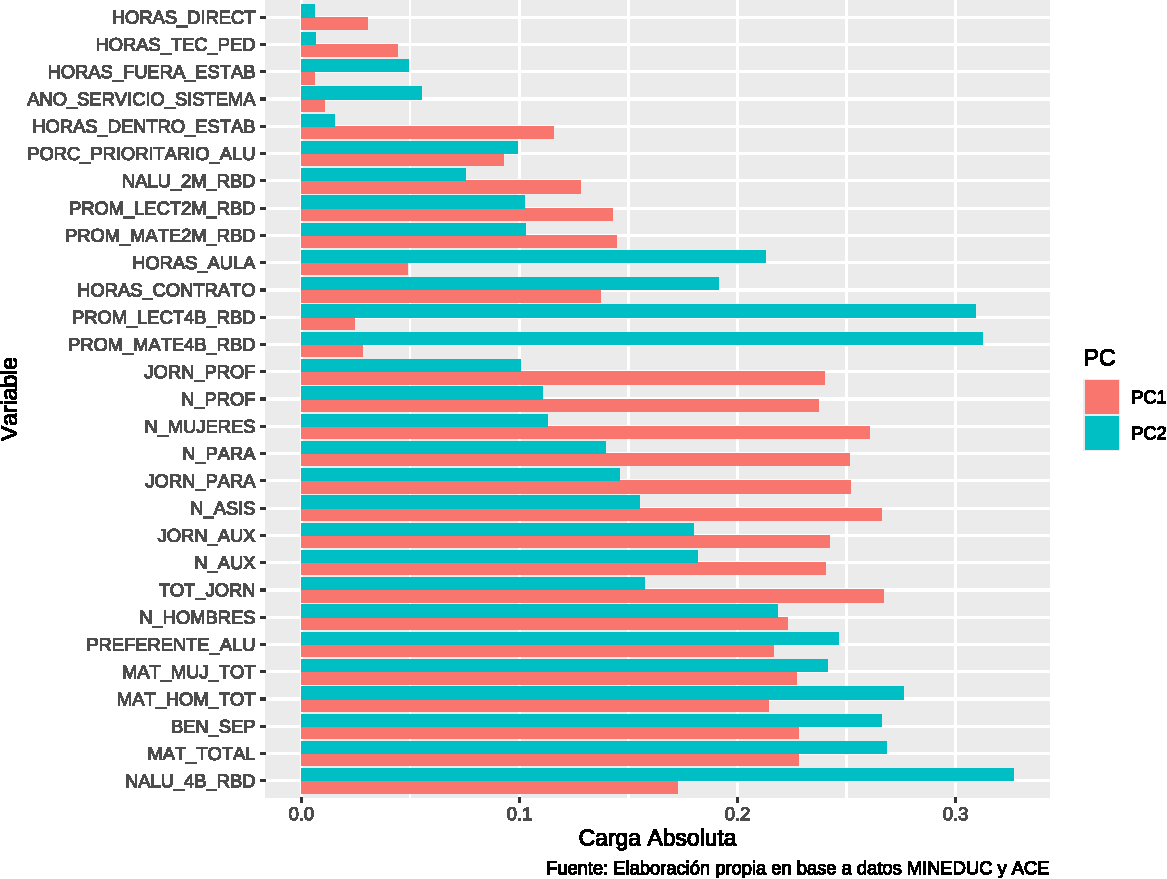
\includegraphics[width=0.8\linewidth,height=6in]{tesis_ver_final_files/figure-latex/anexo-b-1}

\subsection{Anexo C. Ponderación de variables por clúster}\label{anexo-c.-ponderaciuxf3n-de-variables-por-cluxfaster}

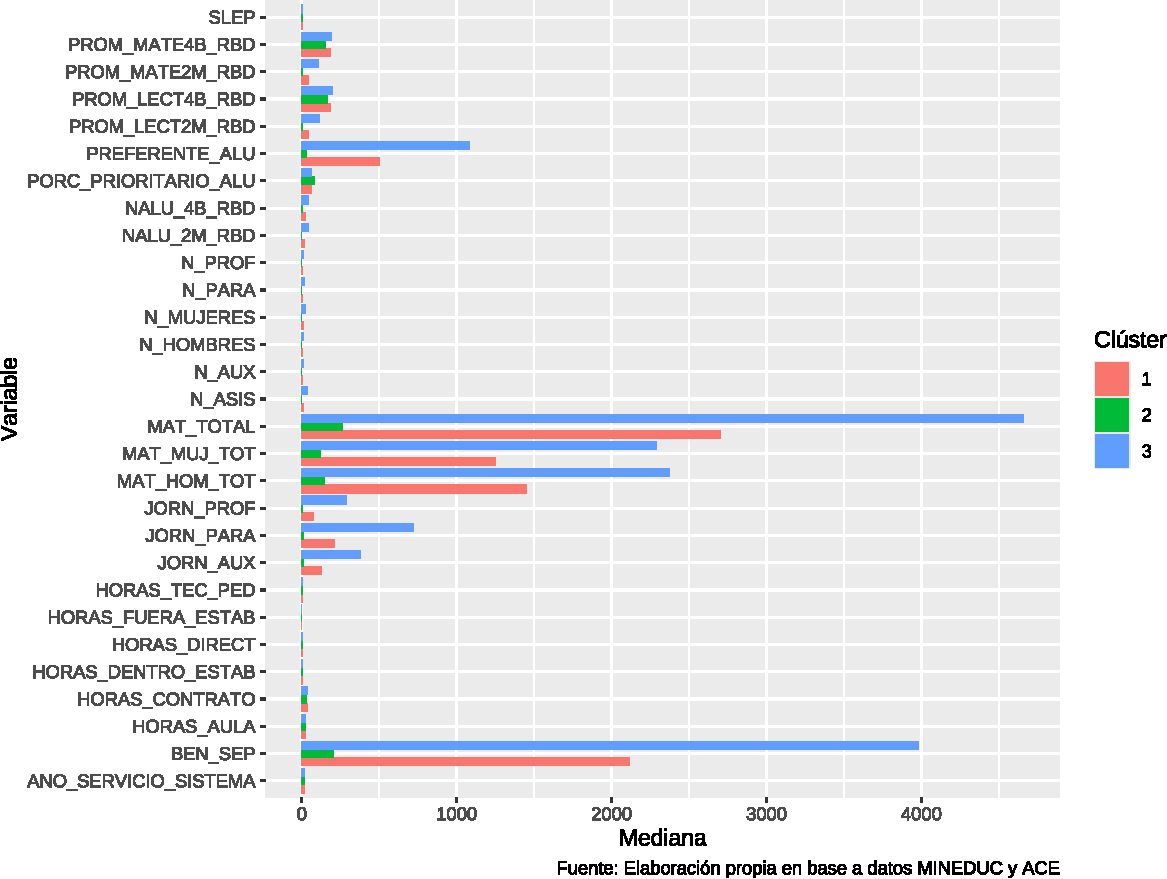
\includegraphics[width=0.8\linewidth,height=6in]{tesis_ver_final_files/figure-latex/anexo-c-1}

\newpage

\subsection{Anexo D. Gráfico de puntaje de silueta por clúster}\label{anexo-d.-gruxe1fico-de-puntaje-de-silueta-por-cluxfaster}

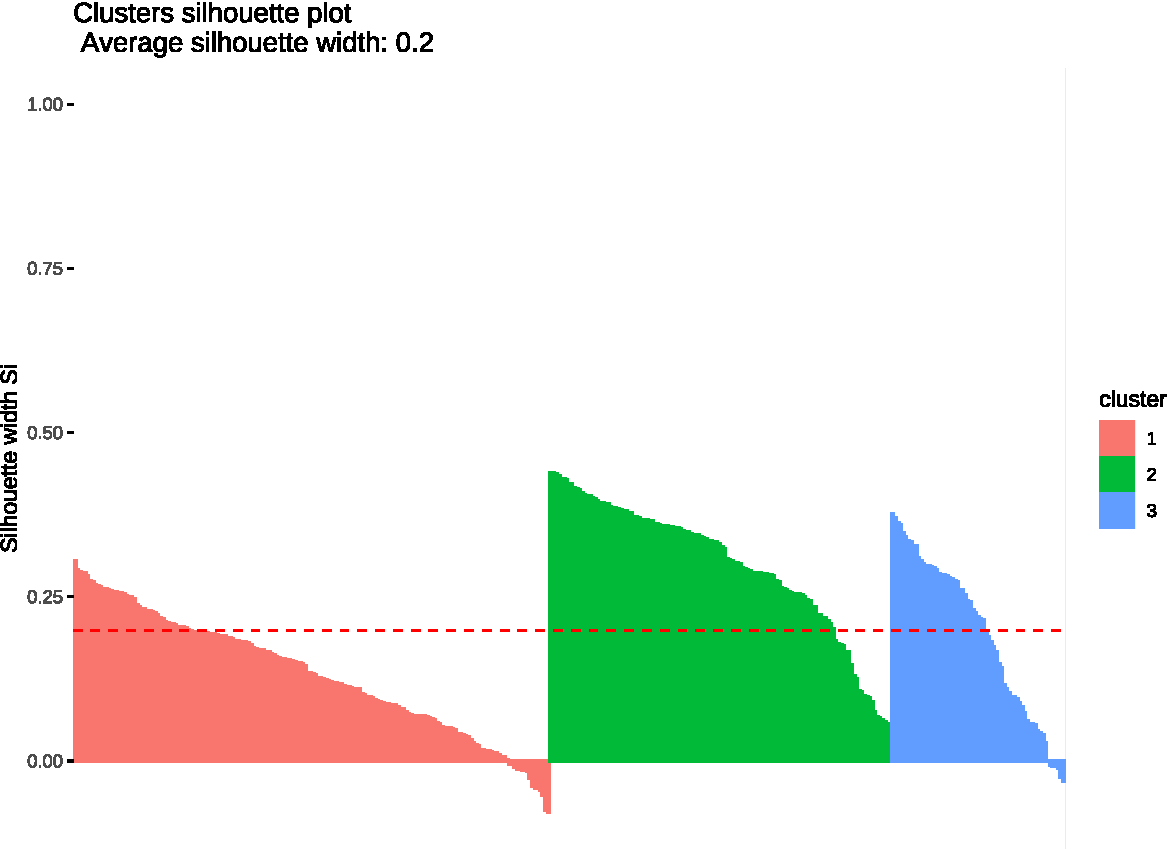
\includegraphics[width=0.8\linewidth,height=6in]{tesis_ver_final_files/figure-latex/anexo-d-1}

\newpage

\end{document}
